\chapter{Kirchhoff-Love shell problem}
\label{chp:chapter5}
\graphicspath{{figures/}{figures/chapter5/}}
\pgfplotsset{
	table/search path={{figures/chapter5/data},{data}},
}

\section{Dual mortar method for non-homogeneous constraints}\label{sec:dual_mortar}

We briefly demonstrate the dual mortar method in the context of an abstract formulation for a constrained problem: find $u\in\mathcal{X}$ and $\lambda\in\mathcal{M}$ such that
\begin{subequations}\label{eq:LM-form}
	\begin{empheq}[left=\empheqlbrace]{alignat=2}
		a(v,u)+b(v,\lambda)&=l(v)\quad &&\forall{}v\in\mathcal{X},\\
		b(\mu,u)&=c(\mu)\quad &&\forall{}\mu\in\mathcal{M},\label{eq:LM-form-constraint}
	\end{empheq}.
\end{subequations}
%%TODO: which section
where $a(\cdot,\cdot)$ is a bilinear form representing a potential energy, $l(\cdot)$ is a linear form representing the external load, $b(\cdot,\cdot)$ is a bilinear form representing a set of constraints on the solution $u$ and $c(\mu)$ is a linear form corresponding to any non-homogeneous constraints. In Section~, $b(\cdot,\cdot)$ and $c(\cdot)$ will represent the continuity constraints across patch boundaries for each Newton-Raphson iteration.

If we introduce a pair of discrete function spaces $\mathcal{X}^h \subset \mathcal{X}$ and $\mathcal{M}^h \subset \mathcal{M}$ we can represent the weak form~\eqref{eq:LM-form} as the matrix problem
\begin{equation}\label{eq:disc-LM-form}
	\mathbf{K}^\text{LM}\mathbf{U}^{\text{LM}}=\begin{bmatrix}
		\mathbf{K} & \mathbf{B}^T \\
		\mathbf{B} & \mathbf{0}
	\end{bmatrix}\mathbf{U}^{\text{LM}}
	=
	\begin{bmatrix}
		\mathbf{F} \\
		\mathbf{R}
	\end{bmatrix},
\end{equation}
where $\mathbf{K}$ is the discretized stiffness matrix, $\mathbf{F}$ is the discretized external force vector, $\mathbf{B}$ is the discretized constraints matrix, $\mathbf{R}$ is the forcing term due to non-homogeneous constraints (for homogeneous constraints, $\mathbf{R} = \mathbf{0}$) and $\mathbf{U}^{\text{LM}}$ is a vector containing the control values $\mathbf{U}$ of the displacement field and the control values $\mathbf{\Lambda}$ Lagrange multiplier field. The mortar method statically condenses out additional unknowns and gives rise to a positive definite variational problem by introducing a constrained function space
\begin{equation}
	\mathcal{V}^h\coloneq\{u^h\in\mathcal{X}^h\, | \, b(\lambda^h,u^h)=0, \quad \forall{}\lambda^h\in\mathcal{M}^h\}.
\end{equation}
The saddle point problem~\eqref{eq:LM-form} can now be transformed into a minimization problem: find a general solution $u^h_\text{hom}\in\mathcal{V}^h$ such that, for $u^h = u^h_\text{hom}+ u^h_\text{non}$
\begin{equation}
	a(v^h, u^h)=l(v^h),\quad \forall{}v^h\in\mathcal{V}^h,
\end{equation}
where $u^h_\text{non}\in \mathcal{X}^h$ is a particular solution that satisfies the constraint~\eqref{eq:LM-form-constraint}. Given $\mathbf{N}^{\mathcal{X}^h}$, the vector containing the basis functions of $\mathcal{X}^h$, the vector containing the basis functions of $\mathcal{V}^h$ is given by
\begin{equation}
	\mathbf{N}^{\mathcal{V}^h}=\left[\mathbf{B}^\perp\right]^T\mathbf{N},\label{eq:basis-null-space}
\end{equation}
where the matrix $\mathbf{B}^\perp$ is the vector basis of the null space of the constraint matrix $\mathbf{B}$. If the Lagrange multiplier space is discretized by a set of dual basis functions, the constraint matrix $\mathbf{B}$ can be written as~\cite{gilbert1987computing}
\begin{equation}\label{eq:constraint-form}
	\mathbf{B}=\begin{bmatrix}
		\mathbf{I} & \mathbf{B_2}
	\end{bmatrix},
\end{equation}
the bandwidth of $\mathbf{B}_2$ depends on the support size of dual basis functions. \par

For a $\mathbf{B}$ in the form~\eqref{eq:constraint-form}, the vector basis of its null space can be obtained from
\begin{equation}
	\mathbf{B}^\perp=\begin{bmatrix}
		-\mathbf{B}_2 \\
		\mathbf{I}
	\end{bmatrix}.
	\label{eq:null-space}
\end{equation}
The discretization of the constraint~\eqref{eq:LM-form-constraint} is
\begin{equation}
	\mathbf{B}\mathbf{U}^\text{non} = \mathbf{R},
\end{equation}
where a particular solution can be solved from~\cite{ainsworth2001essential}
\begin{equation}
	\mathbf{U}^\text{non} = \mathbf{B}^T\left[ \mathbf{B}\mathbf{B}^T \right]^{-1}\mathbf{R}.
\end{equation}
However, for a constraint matrix takes the form~\eqref{eq:constraint-form}, a particular solution can be explicitly constructed as
\begin{equation}
	\mathbf{U}^\text{non} = \begin{bmatrix}
		\mathbf{R} \\\mathbf{0}
	\end{bmatrix}.\label{eq:dual_particular_solution}
\end{equation}
The mortar linear system can now be written as
\begin{equation}
	\mathbf{K}^{\text{mortar}}\mathbf{U}^{\text{mortar}}=\left[\mathbf{B}^\perp\right]^T\mathbf{K}\mathbf{B}^\perp\mathbf{U}^{\text{mortar}}=\left[\mathbf{B}^\perp\right]^T\mathbf{F}-\left[\mathbf{B}^\perp\right]^T\mathbf{K}\mathbf{U}^\text{non}.\label{eq:mortar-form-discretized}
\end{equation}
The relation between the mortar displacement nodal value vector $\mathbf{U}^{\text{mortar}}$, non-homogeneous solution $\mathbf{U}^\text{non}$ and $\mathbf{U}$ is given by
\begin{equation}
	\mathbf{U}=\mathbf{B}^\perp\mathbf{U}^{\text{mortar}}+\mathbf{U}^\text{non}.
\end{equation}
With a sparse $\mathbf{B}^\perp$ obtained from a set of dual basis with compact support, the stiffness matrix of the mortar formulation $\mathbf{K}^{\text{mortar}}$ will remain sparse, resulting in an efficient linear system.

\section{Formulation of Kirchhoff-Love shell}\label{sec:formulation}

In this section, we present the formulation of Kirchhoff-Love shell in compact form. The theory of Kirchhoff-Love shell is based on the assumption that the normal of the shell's mid-surface remains perpendicular in the deformed configuration. Hence, the strain the transverse strains are zero and the description of shell geometry can be reduced to its mid-surface.

\subsection{Kinematics}\label{sec:kinematics}

In what follows, we use Greek letters for indices taking values $\left\{1, 2\right\}$ and Latin letters for $\left\{1,2,3\right\}$, respectively. Einstein summation convention on repeated indices is also utilized. We now consider a shell structure of arbitrary geometry with constant thickness $h$ and parameterized with curvilinear coordinates $\theta^i$, where $\theta^1$ and $\theta^2$ denote the natural curvilinear coordinates and $\theta^3$ indicates the thickness direction with $\theta^3\in \left[-0.5h, \; 0.5h\right]$ (see Figure~\ref{fig:shell_configuration}). We use $\mathbf{R}(\theta^1,\theta^2), \mathbf{r}(\theta^1,\theta^2)\colon \mathbb{R}^2\rightarrow\mathbb{R}^3$ to describe the mid-surface of a shell in reference and current configurations, respectively. For simplicity and without loss of generality, we assume the parametric domain $\hat{\Omega}=[0,1]\times[0,1]$. The displacement of the shell mid-surface is given by
\begin{equation}
	\label{}
	\mathbf{u}(\theta^1,\theta^2) = \mathbf{r}(\theta^1,\theta^2)-\mathbf{R}(\theta^1,\theta^2).
\end{equation}
The mid-surface covariant base vectors in both configurations are obtained by
\begin{equation}
	\label{eq:mid_surface_base_vector}
	\begin{cases}
		\begin{aligned}
			\mathbf{A}_\alpha & =\mathbf{R}_{,\alpha} = \frac{\partial\mathbf{R}}{\partial\theta^\alpha}            \\
			\mathbf{A}_3      & = \frac{\mathbf{A}_1\times\mathbf{A}_2}{\vert{\mathbf{A}_1\times\mathbf{A}_2}\vert}
		\end{aligned}
	\end{cases},\qquad
	\begin{cases}
		\begin{aligned}
			\mathbf{a}_\alpha & =\mathbf{r}_{,\alpha} = \frac{\partial\mathbf{r}}{\partial\theta^\alpha}  =  \mathbf{A}_\alpha+\mathbf{u}_{,\alpha} \\
			\mathbf{a}_3      & = \frac{\mathbf{a}_1\times\mathbf{a}_2}{\vert{\mathbf{a}_1\times\mathbf{a}_2}\vert}
		\end{aligned}
	\end{cases},
\end{equation}
where $\vert\cdot\vert$ denotes the Euclidean length of the given vector. $\mathbf{A}_3$ and $\mathbf{a}_3$ are commonly refered to as the directors in the reference and currect configurations. The position vector of any material point within the shell in both reference configuration and current configuration are described by
\begin{equation}
	\label{eq:position_vector}
	\begin{cases}
		\begin{aligned}
			\mathbf{X}(\theta^1, \theta^2, \theta^3) & = \mathbf{R}(\theta^1, \theta^2) + \theta^3\mathbf{A}_3(\theta^1,\theta^2) \\
			\mathbf{x}(\theta^1, \theta^2, \theta^3) & = \mathbf{r}(\theta^1, \theta^2) + \theta^3\mathbf{a}_3(\theta^1,\theta^2)
		\end{aligned}
	\end{cases},
\end{equation}
Similar to the mid-surface, the covariant base vectors at any arbitrary material point within the shell in two configurations are obtained by
\begin{equation}
	\label{eq:base_vector}
	\begin{cases}
		\begin{aligned}
			\mathbf{G}_\alpha & =\mathbf{X}_{,\alpha} = \mathbf{A}_\alpha+\theta^3\mathbf{A}_{3,\alpha} \\
			\mathbf{G}_3      & = \mathbf{X}_{,3} = \mathbf{A}_3
		\end{aligned}
	\end{cases},\qquad
	\begin{cases}
		\begin{aligned}
			\mathbf{g}_\alpha & =\mathbf{x}_{,\alpha} = \mathbf{a}_\alpha+\theta^3\mathbf{a}_{3,\alpha} \\
			\mathbf{g}_3      & = \mathbf{x}_{,3} = \mathbf{a}_3
		\end{aligned}
	\end{cases}.
\end{equation}


\begin{figure}[h]
	\center
	\includestandalone[scale=1]{configuration}%     without .tex extension
	% or use \input{mytikz}
	\caption{Illustration of deformation, reference and currect configuration of Kirchhoff-Love shell. The mid-surface is denoted by blue color.}
	\label{fig:shell_configuration}
\end{figure}
The covariant and contravariant metric coefficients are computed by
\begin{equation}
	\label{eq:covariant_contravariant_metric}
	\begin{cases}
		\begin{aligned}
			G_{ij} & =\mathbf{G}_i\cdot\mathbf{G}_j \\
			G^{ij} & =\left[G_{ij}\right]^{-1}
		\end{aligned}
	\end{cases},\qquad
	\begin{cases}
		\begin{aligned}
			A_{ij} & =\mathbf{A}_i\cdot\mathbf{A}_j \\
			A^{ij} & =\left[A_{ij}\right]^{-1}
		\end{aligned}
	\end{cases},\qquad
	\begin{cases}
		\begin{aligned}
			g_{ij} & =\mathbf{g}_i\cdot\mathbf{g}_j \\
			g^{ij} & =\left[g_{ij}\right]^{-1}
		\end{aligned}
	\end{cases},\qquad
	\begin{cases}
		\begin{aligned}
			a_{ij} & =\mathbf{a}_i\cdot\mathbf{a}_j \\
			a^{ij} & =\left[a_{ij}\right]^{-1}
		\end{aligned}
	\end{cases}.
\end{equation}
The contravariant base vectors are then given by
\begin{equation}
	\label{eq:contravariant_base_vector}
	\mathbf{G}^i = G^{ij}\mathbf{G}_j,\qquad \mathbf{A}^i = A^{ij}\mathbf{A}_j,\qquad \mathbf{g}^i = g^{ij}\mathbf{g}_j,\qquad \mathbf{a}^i = a^{ij}\mathbf{a}_j.
\end{equation}

Form the numerour strain measures, we use the \textit{Green-Lagrangian} strain tensor to describe the strain, which is defined as
\begin{equation}
	\label{eq:green_lagrangian}
	\mathbf{E} = \frac{1}{2}\left( \mathbf{F}^T\mathbf{F}-\mathbf{I} \right),
\end{equation}
where $\mathbf{F}=\frac{\partial \mathbf{x}}{\partial \mathbf{X}}=\mathbf{g}_i\otimes\mathbf{G}^i$ is the deformation gradient and $\mathbf{I}$ is the identity tensor. Alternatively, $\mathbf{E}$ can be represented as
\begin{equation}
	\label{eq:green_lagrangian_contravariant}
	\mathbf{E}=E_{ij}\mathbf{G}^i\otimes\mathbf{G}^j,\quad\text{with } E_{ij} = \frac{1}{2}\left( g_{ij}-G_{ij} \right).
\end{equation}
Substituting~\eqref{eq:covariant_contravariant_metric} into~\eqref{eq:green_lagrangian_contravariant}, we obtain $E_{i3}=E_{3i}=0$. Separating the strain into a constant part due to membrane load and alinear part due to bending and neglecting $\bigO((\theta^3)^2)$ terms, the rest strain coefficients are given by
\begin{equation}
	\label{}
	E_{\alpha\beta} = \epsilon_{\alpha\beta} + \theta^3\kappa_{\alpha\beta},
\end{equation}
where the membrane strain tensor
\begin{equation}
	\label{eq:membrane_strains}
	\mathbf{\epsilon} = \epsilon_{\alpha\beta}\mathbf{G}^\alpha\otimes\mathbf{G}^\beta, \quad\epsilon_{\alpha\beta} = \frac{1}{2}\left( a_{\alpha\beta}-A_{\alpha\beta} \right) = \frac{1}{2}\left( \mathbf{a}_{\alpha}\cdot\mathbf{a}_{\beta}-\mathbf{A}_{\alpha}\cdot\mathbf{A}_{\beta} \right),
\end{equation}
and the tensor expressing changes in curvature
\begin{equation}
	\label{eq:curvatures}
	\mathbf{\kappa} = \kappa_{\alpha\beta}\mathbf{G}^\alpha\otimes\mathbf{G}^\beta,\quad\kappa_{\alpha\beta} = b_{\alpha\beta}-B_{\alpha\beta},\qquad\text{with }
	\begin{cases}
		\begin{aligned}
			B_{\alpha\beta} & =\frac{1}{2}\left( \mathbf{A}_{\alpha}\cdot\mathbf{A}_{3,\beta}+\mathbf{A}_{\beta}\cdot\mathbf{A}_{3,\alpha}\right) = -\mathbf{A}_{\alpha,\beta}\cdot\mathbf{A}_3 \\
			b_{\alpha\beta} & =\frac{1}{2}\left( \mathbf{a}_{\alpha}\cdot\mathbf{a}_{3,\beta}+\mathbf{a}_{\beta}\cdot\mathbf{a}_{3,\alpha}\right)  =-\mathbf{a}_{\alpha,\beta}\cdot\mathbf{a}_3
		\end{aligned}
	\end{cases}.
\end{equation}

\subsection{Equilibrium of elastic Kirchhoff-Love shell}\label{sec:equilibrium}

Next, we develop the variational formulation from the minimization of the potential energy. For the sake of simplicity, we assume that the shell is linear elastic with a strain energy density per unit area of the form~\cite{chapelle2010finite}
\begin{equation}
	\label{eq:strain_energy_density}
	W(\theta^1,\theta^2) = \frac{1}{2}\left( h \mathbf{\epsilon}\colon \mathbf{C}\colon \mathbf{\epsilon} + \frac{h^3}{12} \mathbf{\kappa }\colon \mathbf{C}\colon \mathbf{\kappa } \right)= \frac{1}{2}\left( hC^{\alpha\beta\gamma\delta}\epsilon_{\alpha\beta}\epsilon_{\gamma\delta}+\frac{h^3}{12}C^{\alpha\beta\gamma\delta}\kappa_{\alpha\beta}\kappa_{\gamma\delta} \right),
\end{equation}
where $E$ is Young's modulus, $\nu$ is Poisson's ratio and the fourth order material tensor
\begin{equation}
	\label{eq:material_tensor}
	\mathbf{C} = C^{\alpha\beta\gamma\delta} \mathbf{A}_\alpha\otimes\mathbf{A}_\beta\otimes\mathbf{A}_\gamma\otimes\mathbf{A}_\delta,\qquad C^{\alpha\beta\gamma\delta} = \frac{E\nu}{1-\nu^2} A^{\alpha\beta}A^{\gamma\delta}+\frac{E}{2(1+\nu)}\left( A^{\alpha\gamma}A^{\beta\delta}+A^{\alpha\delta}A^{\beta\gamma} \right).
\end{equation}
The membrane force resultants tensor and the bending moment resultants tensor read
\begin{equation}
	\label{eq:stress_and_moment}
	\begin{cases}
		\begin{aligned}
			\mathbf{n} & = n^{\alpha\beta}\mathbf{A}_\alpha\otimes\mathbf{A}_\beta,\quad n^{\alpha\beta} =\frac{\partial W}{\partial \epsilon_{\alpha\beta}} = hC^{\alpha\beta\gamma\delta}\epsilon_{\gamma\delta}         \\
			\mathbf{m} & = m^{\alpha\beta}\mathbf{A}_\alpha\otimes\mathbf{A}_\beta,\quad m^{\alpha\beta} =\frac{\partial W}{\partial \kappa_{\alpha\beta}} =\frac{h^3}{12}C^{\alpha\beta\gamma\delta}\kappa_{\gamma\delta}
		\end{aligned}
	\end{cases}.
\end{equation}
The potential energy of Kirchhoff-Love shell is defined as
\begin{equation}
	\label{eq:potential_energy}
	\Pi(\mathbf{u},\mathbf{u}) = \Pi^\text{int}(\mathbf{u},\mathbf{u})+\Pi^\text{ext}(\mathbf{f}, \mathbf{u}) = \int_{\overline{\Omega}}W d\Omega+\Pi^\text{ext}(\mathbf{f}, \mathbf{u}),
\end{equation}
where $\overline{\Omega}$ is the mid-surface of the shell in the reference configuration, $d\Omega=\vert{\mathbf{A}_1\times\mathbf{A}_2}\vert d\theta^1 d\theta^2$ is the differential area, $\Pi^\text{int}(\mathbf{u},\mathbf{u}) = \int_{\overline{\Omega}}W d\Omega$ is the strain energy and $\Pi^\text{ext}(\mathbf{f},\mathbf{u})$ is the external work due to external force $\mathbf{f}$, in general $\Pi^\text{ext}$ is a linear functional with respect to $\mathbf{u}$. The variation formulation can be obtained from the minimization of the potential energy,
\begin{equation}
	\label{eq:weak_form_nonlinear}
	\delta \Pi(\mathbf{u},\delta\mathbf{u}) = \frac{\partial \Pi}{\partial \mathbf{u}} \delta\mathbf{u} = \int_{\overline{\Omega}} \left(\delta{\epsilon(\mathbf{u},\delta\mathbf{u})} \colon\mathbf{n}(\mathbf{u}) + \delta{\kappa(\mathbf{u},\delta\mathbf{u})} \colon \mathbf{m}(\mathbf{u}) \right)d \Omega+\Pi^\text{ext}(\mathbf{f},\delta\mathbf{u})= 0,
\end{equation}
with
\begin{equation}
	\label{}
	\delta{\epsilon(\mathbf{u},\delta\mathbf{u})} = \frac{\partial \mathbf{\epsilon}(\mathbf{u})}{\partial \mathbf{u}}\delta\mathbf{u},\qquad \text{and }\delta{\kappa(\mathbf{u},\delta\mathbf{u})} = \frac{\partial \mathbf{\kappa}(\mathbf{u})}{\partial \mathbf{u}}\delta\mathbf{u}.
\end{equation}
However, the variational formulation~\eqref{eq:weak_form_nonlinear} is a nonlinear functional with respect to $\mathbf{u}$ and cannot be solved directly. Hence, we adopt the Newton-Raphson method to solve the problem iteratively. Assuming $\mathbf{u}^{i+1} = \mathbf{u}^{i} +{\Delta} \mathbf{u}$, the weak form for solving ${\Delta} \mathbf{u}$ is stated as: find ${\Delta}\mathbf{u}\in \boldsymbol{\mathcal{X}}$, such that
\begin{equation}
	\label{eq:weak_form_linearized}
	\left(K_\text{m}(\mathbf{u}^i,\delta\mathbf{u},\Delta\mathbf{u})+K_\text{b}(\mathbf{u}^i,\delta\mathbf{u},\Delta\mathbf{u})\right)=-\delta \Pi(\mathbf{u}^{i},\delta\mathbf{u}),\qquad \forall \delta\mathbf{u}\in \boldsymbol{\mathcal{X}},
	% -\int_\Omega \left(\delta{\epsilon(\mathbf{u}_{i},\delta\mathbf{u})} \colon \delta\mathbf{n}(\mathbf{u}_i,{\Delta}\mathbf{u}) + \delta{\epsilon(\mathbf{u}_{i},\delta\mathbf{u},\Delta\mathbf{u})} \colon \mathbf{n}(\mathbf{u}_i) + \delta{\kappa(\mathbf{u}_i,\delta\mathbf{u})} \colon \delta\mathbf{m}(\mathbf{u}_i,{\Delta}\mathbf{u}) \right)d \Omega = \delta \Pi(\mathbf{u}_{i},\delta\mathbf{u}),\qquad \forall \delta\mathbf{u}\in \mathbf{\mathcal{U}},
\end{equation}
where $i$ denotes the iterative step, the solution space $\boldsymbol{\mathcal{X}}=\left[H^2(\hat{\Omega})\right]^3$, the membrane stiffness
\begin{equation}
	K_\text{m}(\mathbf{u}^i,\delta\mathbf{u},\Delta\mathbf{u}) = \int_{\overline{\Omega}} \delta{\epsilon(\mathbf{u}^{i},\delta\mathbf{u})} \colon \delta\mathbf{n}(\mathbf{u}^i,{\Delta}\mathbf{u}) + \delta{\epsilon(\mathbf{u}^{i},\delta\mathbf{u},\Delta\mathbf{u})} \colon \mathbf{n}(\mathbf{u}^i) d\Omega,
\end{equation}
and the bending stiffness
\begin{equation}
	K_\text{b}(\mathbf{u}^i,\delta\mathbf{u},\Delta\mathbf{u}) = \int_{\overline{\Omega}} \delta{\kappa(\mathbf{u}^{i},\delta\mathbf{u})} \colon \delta\mathbf{m}(\mathbf{u}^i,{\Delta}\mathbf{u}) + \delta{\kappa(\mathbf{u}^{i},\delta\mathbf{u},\Delta\mathbf{u})} \colon \mathbf{m}(\mathbf{u}^i) d\Omega,
\end{equation}
with
\begin{equation}
	\begin{cases}
		\begin{aligned}
			\delta{\mathbf{n}(\mathbf{u},{\Delta}\mathbf{u})}              & = \frac{\partial \mathbf{n}(\mathbf{u})}{\partial \mathbf{u}}{\Delta}\mathbf{u} = h\mathbf{C}\colon \delta\mathbf{\epsilon}(\mathbf{u},\Delta\mathbf{u}), \\
			\delta{\mathbf{m}({\Delta}\mathbf{u})}                         & = \frac{\partial \mathbf{m}}{\partial \mathbf{u}}{\Delta}\mathbf{u} = \frac{h^3}{12}\mathbf{C}\colon \delta\mathbf{\kappa}(\Delta\mathbf{u}),             \\
			\delta{\epsilon(\mathbf{u},\delta\mathbf{u},\Delta\mathbf{u})} & = \frac{\partial \delta\mathbf{\epsilon}(\mathbf{u},\delta\mathbf{u})}{\partial \mathbf{u}}\Delta\mathbf{u},                                              \\
			\delta{\kappa(\mathbf{u},\delta\mathbf{u},\Delta\mathbf{u})}   & = \frac{\partial \delta\mathbf{\kappa}(\mathbf{u},\delta\mathbf{u})}{\partial \mathbf{u}}\Delta\mathbf{u}.
		\end{aligned}
	\end{cases}
\end{equation}

\section{A dual mortar formulation for the multi-patch Kirchhoff-Love shell}\label{sec:multi_patch}

Most of the commonly used patch coupling approaches for Kirchhoff-Love shell fall into the following categories: penalty method~\cite{kiendl2010bending, herrema2019penalty}, Lagrange multiplier method (collocation approach can be viewed as a Lagrange multiplier method with the Lagrange multiplier discretized by Dirac delta functions )~\cite{coox2017flexible, hirschler2019embedded, schuss2019multi, goyal2017penalty}, and Nitsche's method~\cite{guo_nitsches_2015, nguyen2017isogeometric}. The performance of the penalty method is significantly influenced by the choice of the penalty parameter: a small penalty parameter cannot effectively enforce inter-patch constraint while a large penalty parameter may badly affect the condition number of the linear system. Usually, the selection of the penalty parameter is performed empirically by the analyst. The Lagrange multiplier methods leads to a saddle point problem, for with iterative methods are known to be less efficient than for symmetric positive definite systems. In addition, redundancy may happen in the discretized constraint matrix, leading to a rank deficiency linear system (\textit{inf-sup} instability). Although a global factorization followed by a static condensation can circumvent this issue, the resulted linear system no longer preserves its sparsity and may be polluted by the numerical error within the factorization process. The stability parameter in the Nitsche method needs to be approximated by eigenvalue problems associated with element intersections, which increase the computational cost. For nonlinear problems, the Nitsche's method becomes complex as it requires the tractions and their variations on the interface. \par

Here, we present a dual mortar formulation for the Kirchhoff-Love shell over multi-patch tensor product domains. Thanks to the locally supported dual basis, the linear system can be statically condensed with minimum computational cost and the resulted linear system preserves its sparsity. Along each interface, we introduce a local coordinate system, in which a generic inter-patch constraint is developed in a natural manner. The main advantages of this generic inter-patch constraint are that it deals with both patches joining smoothly and those joining at a kink in a uniform framework and it is compatible with dual basis.\par

We first introduce a rotation operator: for a vector $\mathbf{v}\in\mathbb{R}^3$, its rotation round the axis $\mathbf{k}\in\mathbb{R}^3$ by an angle $\theta$ according to the right hand rule is given as
\begin{equation}
	\mathbf{R}_{\mathbf{k},\theta}(\mathbf{v}) = \mathbf{v}\cos(\theta)+\left(\frac{\mathbf{k}}{\vert \mathbf{k} \vert}\times \mathbf{v}\right)\sin(\theta)+\frac{\mathbf{k}}{\vert \mathbf{k} \vert}\left(\frac{\mathbf{k}}{\vert \mathbf{k} \vert}\cdot\mathbf{v}\right)(1-\cos(\theta)). \label{eq:rodrigues_rotation}
\end{equation}
This operator is called the Rodrigues' rotation formula~\cite{rodrigues1840lois} and will play an important rule in formulating the inter-patch constraint.\par

To demonstrate our approach, we consider a kinked shell structure consisting of two NURBS patches shown in Figure~\ref{fig:two_patch_shell_with_kink}. We denote by $\Omega_s$ the slave domain, $\Omega_m$ the master domain and $\Gamma_{sm}$ the intersection between two patches. These two domains are parameterized by coordinate systems $(\theta^1_s, \theta^2_s)$ and $(\theta^1_m, \theta^2_m)$, respectively.

\begin{figure}[ht]
	\center
	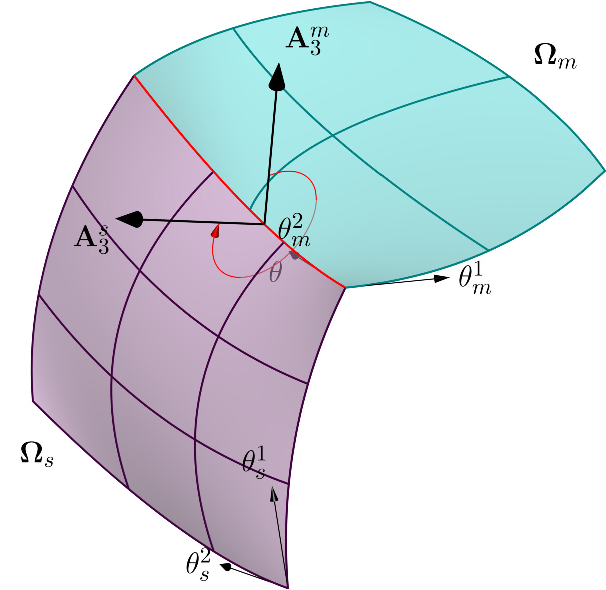
\includegraphics[width=.5\columnwidth]{two_patch_shell_with_kink}
	\caption{A two-patch non-conforming Kirchhoff-Love shell consisting of two patches $\Omega_s$ and $\Omega_m$ with the intersection denoted by the red curve. The director $\mathbf{A}_3^m$ of $\Omega_m$ and the director $\mathbf{A}_3^s$ of $\Omega_s$ determine a rotation angle $\theta$ along the intersection. }\label{fig:two_patch_shell_with_kink}
\end{figure}

\subsection{A local coordinate system for patch intersections}

\begin{table}
	\center
	\caption{The strategy in selecting the restrictions of $\bar{\theta}^1$ and $\bar{\theta}^2$ on $\Omega_s$, where $\bar{\mathbf{A}}_\alpha^k=\sfrac{\partial\mathbf{X}^k}{\partial \bar{\theta}^\alpha\vert_{\Omega_k}}$}
	\label{tab:orientation_and_coordinate}
	\begin{tabularx}{.5\textwidth}{l@{\extracolsep{\fill}}cc}
		\toprule
		Interface orientation & $\bar{\theta}^1\vert_{\Omega_s}$         & $\bar{\theta}^2\vert_{\Omega_s}$         \\
		\midrule
		South                 & $\bar{\mathbf{A}}_1^s = -\mathbf{A}_2^s$ & $\bar{\mathbf{A}}_2^s = \mathbf{A}_1^s$  \\
		East                  & $\bar{\mathbf{A}}_1^s = \mathbf{A}_1^s$  & $\bar{\mathbf{A}}_2^s = \mathbf{A}_2^s$  \\
		North                 & $\bar{\mathbf{A}}_1^s = \mathbf{A}_2^s$  & $\bar{\mathbf{A}}_2^s = -\mathbf{A}_1^s$ \\
		West                  & $\bar{\mathbf{A}}_1^s = -\mathbf{A}_1^s$ & $\bar{\mathbf{A}}_2^s = -\mathbf{A}_2^s$ \\
		\bottomrule
	\end{tabularx}
\end{table}

In this subsection, we reparameterize the intersection between the slave patch and the master patch by a coordinate system $(\bar{\theta}^1, \bar{\theta}^2)$. However, we do not need to develop explicitly the map from $(\bar{\theta}^1, \bar{\theta}^2)$ to $\Omega_s$ and $\Omega_m$. Instead, we are interested in the covariant base vectors $(\bar{\mathbf{A}}_1, \bar{\mathbf{A}}_2)$ defined in the new coordinate system and how they behave during the deformation. The new coordinate system is defined based on the orientation of both the slave patch and the master path. We first specify the restrictions of $\bar{\theta}^1$ and $\bar{\theta}^2$ on $\Omega_s$ following the strategy given in Table~\ref{tab:orientation_and_coordinate}. For example, if an intersection is a north edge on the slave patch, we have
\begin{equation}
	\left\{
	\begin{split}
		\bar{\mathbf{A}}^s_1 &= \frac{\partial\mathbf{X}^s}{\partial \bar{\theta}^1\vert_{\Omega_s}} = \begin{bmatrix}
			\mathbf{A}_1^s & \mathbf{A}_2^s
		\end{bmatrix} \cdot \mathbf{J}_{\bar{\theta}^1}\vert_{\Omega_s} = \mathbf{A}_2^s\\
		\bar{\mathbf{A}}_2^s &= \frac{\partial\mathbf{X}^s}{\partial \bar{\theta}^2\vert_{\Omega_s}} = \begin{bmatrix}
			\mathbf{A}_1^s & \mathbf{A}_2^s
		\end{bmatrix} \cdot \mathbf{J}_{\bar{\theta}^2}\vert_{\Omega_s} = -\mathbf{A}_1^s
	\end{split}
	\right.,
\end{equation}
with
\begin{equation}
	\left\{
	\begin{split}
		\mathbf{J}_{\bar{\theta}^1}\vert_{\Omega_s} &=
		\begin{bmatrix}
			\frac{\partial \theta^1_s}{\partial \bar{\theta}^1\vert_{\Omega_s}} \\
			\frac{\partial \theta^2_s}{\partial \bar{\theta}^1\vert_{\Omega_s}}
		\end{bmatrix}=
		\begin{bmatrix}
			0 \\
			1
		\end{bmatrix}\\
		\mathbf{J}_{\bar{\theta}^2}\vert_{\Omega_s} &= \begin{bmatrix}
			\frac{\partial \theta^1_s}{\partial \bar{\theta}^2\vert_{\Omega_s}} \\
			\frac{\partial \theta^2_s}{\partial \bar{\theta}^2\vert_{\Omega_s}}
		\end{bmatrix}=
		\begin{bmatrix}
			-1 \\
			0
		\end{bmatrix}
	\end{split}
	\right..
\end{equation}

For different pairings of the slave edge and the master edge, the corresponding Jacobian $\mathbf{J}_{\bar{\theta}^1}\vert_{\Omega_s}$, $\mathbf{J}_{\bar{\theta}^2}\vert_{\Omega_s}$ can be computed in the same manner. \par

We now extend the curvilinear coordinate system $(\bar{\theta}^1, \bar{\theta}^2)$ from the slave patch to the master patch. A natural choice of the restriction of $\bar{\theta}^2$ on $\Omega_m$ is
\begin{equation}
	\bar{\theta}^2\vert_{\Omega_m}=\bar{\theta}^2\vert_{\Omega_s}, \text{ or } \bar{\mathbf{A}}^m_2=\bar{\mathbf{A}}^s_2.
\end{equation}
Given the directors $\mathbf{A}^s_3$ and $\mathbf{A}^m_3$ and the axis $\bar{\mathbf{A}}^s_2$, we can now uniquely determine the counterclockwise rotation (see Figure~\ref{fig:two_patch_shell_with_kink}) from $\mathbf{A}^m_3$ to $\mathbf{A}^s_3$ by
\begin{equation}
	\left\{
	\begin{split}
		\cos{\theta} &= \mathbf{A}^m_3\cdot \mathbf{A}^s_3\\
		\sin{\theta} &= \frac{(\bar{\mathbf{A}}^m_2 \times \mathbf{A}^m_3) \cdot \mathbf{A}^s_3}{\vert \bar{\mathbf{A}}^m_2 \vert}.
	\end{split}
	\right.\label{eq:rotation_angle}
\end{equation}
By Equation~\eqref{eq:rodrigues_rotation}, we can define a rotation operator rotate $\mathbf{A}^s_3$ to $\mathbf{A}^m_3$ around the axis $\bar{\mathbf{A}}^m_2$ as
\begin{equation}
	\mathbf{A}^m_3 = \mathbf{R}_{\bar{\mathbf{A}}^m_2,-\theta}(\mathbf{A}^s_3) =  -\mathbf{R}_{\bar{\mathbf{A}}^m_2,\theta}(\mathbf{A}^s_3).
\end{equation}
Meanwhile, the rotation operator $\mathbf{R}_{\bar{\mathbf{A}}^m_2,-\theta}$ also rotates $\bar{\mathbf{A}}^s_1$ to the tangential plane of $\Omega_m$ along the intersection. We let
\begin{equation}
	\bar{\mathbf{A}}^m_1=\mathbf{R}_{\bar{\mathbf{A}}^m_2,-\theta}(\bar{\mathbf{A}}^s_1).\label{eq:reference_constraint_c1}
\end{equation}
The corresponding Jacobians $\mathbf{J}_{\bar{\theta}^1}\vert_{\Omega_m} = \begin{bmatrix}
		\frac{\partial \theta^1_m}{\partial \bar{\theta}^1\vert_{\Omega_m}} & \frac{\partial \theta^2_m}{\partial \bar{\theta}^1\vert_{\Omega_m}}
	\end{bmatrix}^T$ and $\mathbf{J}_{\bar{\theta}^2}\vert_{\Omega_m} = \begin{bmatrix}
		\frac{\partial \theta^1_m}{\partial \bar{\theta}^2\vert_{\Omega_m}} & \frac{\partial \theta^2_m}{\partial \bar{\theta}^2\vert_{\Omega_m}}
	\end{bmatrix}^T$ are given by
\begin{equation}
	\begin{split}
		\begin{bmatrix}
			\mathbf{A}_1^m & \mathbf{A}_2^m
		\end{bmatrix} \cdot \mathbf{J}_{\bar{\theta}^1}\vert_{\Omega_m} &= \mathbf{R}_{\bar{\mathbf{A}}^m_2,-\theta}(\bar{\mathbf{A}}^s_1),\\
		\begin{bmatrix}
			\mathbf{A}_1^m & \mathbf{A}_2^m
		\end{bmatrix} \cdot \mathbf{J}_{\bar{\theta}^2}\vert_{\Omega_m} &= \bar{\mathbf{A}}^s_2.
	\end{split}\label{eq:jacobian_of_Jtheta}
\end{equation}
As $\begin{bmatrix}
		\mathbf{A}_1^m & \mathbf{A}_2^m
	\end{bmatrix}$ is a $3\times 2$ matrix, Equation~\eqref{eq:jacobian_of_Jtheta} could not be factorized directly. However, as $\mathbf{R}_{\bar{\mathbf{A}}^m_2,-\theta}(\bar{\mathbf{A}}^s_1)$ and $\bar{\mathbf{A}}^s_2$ are on the tangential plane of $\Omega_m$, we can solve $\mathbf{J}_{\bar{\theta}^1}\vert_{\Omega_m}$ and $\mathbf{J}_{\bar{\theta}^2}\vert_{\Omega_m}$ by
\begin{equation}
	\begin{split}
		\mathbf{J}_{\bar{\theta}^1}\vert_{\Omega_m} &= \left(\begin{bmatrix}
			\mathbf{A}_1^m & \mathbf{A}_2^m
		\end{bmatrix}^T\cdot\begin{bmatrix}
			\mathbf{A}_1^m & \mathbf{A}_2^m
		\end{bmatrix}\right)^{-1}\left(\begin{bmatrix}
			\mathbf{A}_1^m & \mathbf{A}_2^m
		\end{bmatrix}^T\cdot\mathbf{R}_{\bar{\mathbf{A}}^m_2,-\theta}(\bar{\mathbf{A}}^s_1) \right),\\
		\mathbf{J}_{\bar{\theta}^2}\vert_{\Omega_m} &= \left(\begin{bmatrix}
			\mathbf{A}_1^m & \mathbf{A}_2^m
		\end{bmatrix}^T\cdot\begin{bmatrix}
			\mathbf{A}_1^m & \mathbf{A}_2^m
		\end{bmatrix}\right)^{-1}\left(\begin{bmatrix}
			\mathbf{A}_1^m & \mathbf{A}_2^m
		\end{bmatrix}^T\cdot\bar{\mathbf{A}}^s_2 \right).
	\end{split}
\end{equation}

Following the above procedures, we have that the covariant base vectors of the master patch are nothing but the rotation of the covariant base vectors of the slave patch via the rotation operator $\mathbf{R}_{\bar{\mathbf{A}}^m_2,-\theta}$ (see Figure~\ref{fig:coordinate_system_on_each_patch}), as
\begin{equation}
	\begin{bmatrix}
		\bar{\mathbf{A}}_1^m & \bar{\mathbf{A}}_2^m
	\end{bmatrix}
	=
	\begin{bmatrix}
		\mathbf{R}_{\bar{\mathbf{A}}^m_2,-\theta}(\bar{\mathbf{A}}_1^s) & \bar{\mathbf{A}}_2^s
	\end{bmatrix}
	=
	\mathbf{R}_{\bar{\mathbf{A}}^m_2,-\theta}
	\begin{bmatrix}
		\bar{\mathbf{A}}_1^s & \bar{\mathbf{A}}_2^s
	\end{bmatrix}.
\end{equation}

The partial derivatives of the displacement $\mathbf{u}$ w.r.t. the new coordinate system $(\bar{\theta}^1, \bar{\theta}^2)$ are now given by
\begin{equation}
	\left\{
	\begin{split}
		\bar{\mathbf{u}}^s_{,1} &= \frac{\partial \mathbf{u}^s}{\partial \bar{\theta}^1\vert_{\Omega_s}} = \begin{bmatrix}
			\mathbf{u}^s_{,1} & \mathbf{u}^s_{,2}
		\end{bmatrix}\mathbf{J}_{\bar{\theta}^1}\vert_{\Omega_s}\\
		\bar{\mathbf{u}}^m_{,1} &= \frac{\partial \mathbf{u}^m}{\partial \bar{\theta}^1\vert_{\Omega_m}} = \begin{bmatrix}
			\mathbf{u}^m_{,1} & \mathbf{u}^m_{,2}
		\end{bmatrix}\mathbf{J}_{\bar{\theta}^1}\vert_{\Omega_m}\\
		\bar{\mathbf{u}}^m_{,2} &= \frac{\partial \mathbf{u}^m}{\partial \bar{\theta}^2\vert_{\Omega_m}} = \begin{bmatrix}
			\mathbf{u}^m_{,1} & \mathbf{u}^m_{,2}
		\end{bmatrix}\mathbf{J}_{\bar{\theta}^2}\vert_{\Omega_m}
	\end{split}
	\right..
\end{equation}

\begin{figure}[ht]
	\centering
	\begin{subfigure}[t]{0.4\textwidth}
		\centering
		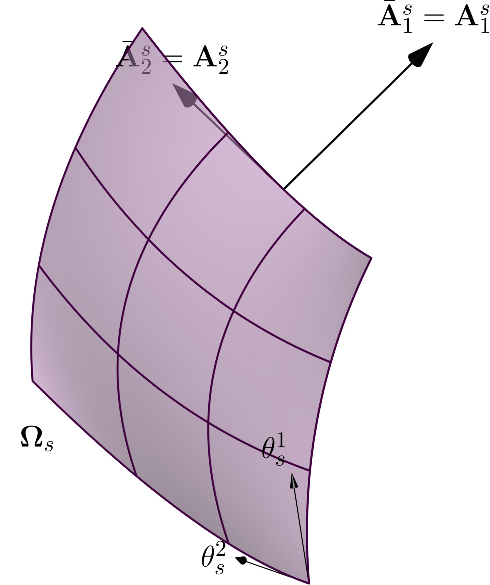
\includegraphics[scale = .7]{master_patch}
		\caption{Slave patch}
	\end{subfigure}
	\begin{subfigure}[t]{0.58\textwidth}
		\centering
		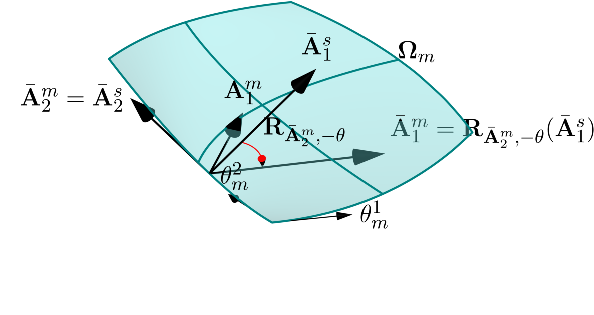
\includegraphics[trim=.2cm .5cm 0 0, clip, scale = .9]{slave_patch}
		\caption{Master patch}
	\end{subfigure}
	\caption{ The covariant base vectors $(\bar{\mathbf{A}}_1, \bar{\mathbf{A}}_2)$ of the coordinate system $(\bar{\theta}^1, \bar{\theta}^2)$ on both the slave patch and the master patch. Note that the covariant base vectors of the master patch can be obtained by rotating the covariant base vectors of the slave patch via the rotation operator $\mathbf{R}_{\bar{\mathbf{A}}^m_2,-\theta}$. }\label{fig:coordinate_system_on_each_patch}
\end{figure}

\begin{remark}
	Following the strategy in Table~\ref{tab:orientation_and_coordinate} is of crucial importance with respect to the algorithm's stability. Figure~\ref{fig:parametric_of_slave_master} shows the restriction of the new coordinate system on the coupling edges for different coupling scenarios. As can be seen, the new coordinate system always follows the right hand rule. On the slave patch, $\bar{\theta}^1$ is always perpendicular to $\bar{\theta}^2$, while on the master patch, $\bar{\theta}^1$ and $\bar{\theta}^2$ forms an angle in the range of $(0^{\circ}, 180^{\circ})$. Thus, the director of the new coordinate system is always consistent with the director of the original coordinate system, i.e.
	\begin{equation}
		\left\{
		\begin{split}
			\bar{\mathbf{A}}^s_3 &= {\mathbf{A}}^s_3\\
			\bar{\mathbf{A}}^m_3 &= {\mathbf{A}}^m_3
		\end{split}
		\right..\label{eq:A3_consistency}
	\end{equation}
	On the contrary, if we do not follow the scheme in Table~\ref{tab:orientation_and_coordinate}, the new coordinate system may not obey the right hand rule, Equation~\eqref{eq:A3_consistency} may not be satisfied and the rotation angle from Equation~\eqref{eq:rotation_angle} may not necessarily guide $\bar{\mathbf{A}}^s_1$ to the tangential plane of $\Omega_m$.
\end{remark}

\begin{figure}[ht]
	\centering
	\begin{subfigure}[b]{0.47\textwidth}
		\centering
		\includestandalone[scale=.9]{master_coordinates}
		\caption{Parametric domain of the master patch}
	\end{subfigure}
	\begin{subfigure}[b]{0.47\textwidth}
		\centering
		\includestandalone[scale=.9]{slave_coordinates}
		\caption{Parametric domain of the slave patch}
	\end{subfigure}
	\caption{The new coordinate system $(\bar{\theta}^1, \bar{\theta}^2)$ on parametric domains of both slave patch and master patch. Coordinate systems on different edges denote the orientations in different coupling scenarios. Note that no matter which edge is coupled, the new coordinate system always obey the right hand rule on both slave and master patches.}
	\label{fig:parametric_of_slave_master}
\end{figure}

\subsection{Generic dual-compatible constraints for Kirchhoff-Love shell coupling}

Shell patches can be coupled smoothly as well as joined at a kink. In this subsection, we propose a set of constraints that can tackle shell coupling in a systematic manner. Compared with existing Kirchhoff-Love shell continuity constraints, the proposed formulation has its uniqueness. For instance, the constraint proposed in~\cite{schuss2019multi} only deal with $G^1$ continuity of adjacent patches, while the proposed formulation can tackle shell patches joined at different angle in a uniform framework. When patches are coupled smoothly, the proposed constraints will enforce $C^1$ continuity across adjacent patches while the angle between directors of adjacent patches will be preserved when they are joined at a kink. The constraint presented in~\cite{coox_robust_2017, hirschler2019embedded} is designed for small deformation problems, while the proposed formulation solves both small deformation and large deformation problems. In addition, the proposed constraints are compatible with dual basis, i.e. the discretized constraint matrix takes the form of Equation~\eqref{eq:constraint-form}, and the \textit{inf-sup} stability is automatically satisfied.\par

In the coordinate system $(\bar{\theta}^1, \bar{\theta}^2)$, two physical properties that satisfied in the reference configuration should be preserved:
\begin{subequations}
	\begin{align}
		\mathbf{X}^s-\mathbf{X}^m=0\quad                                                              & \Rightarrow\quad \mathbf{x}^s-\mathbf{x}^m=0,\label{eq:preserve_c0}                                                               \\
		\bar{\mathbf{A}}^s_3 - \mathbf{R}_{\bar{\mathbf{A}}^m_2,\theta}(\bar{\mathbf{A}}^m_3)=0 \quad & \Rightarrow\quad \bar{\mathbf{a}}^s_3 - \mathbf{R}_{\bar{\mathbf{a}}^m_2,\theta}(\bar{\mathbf{a}}^m_3) = 0,\label{eq:preserve_c1}
	\end{align}
\end{subequations}
where Equation~\eqref{eq:preserve_c0} indicates the continuity of the displacement and Equation~\eqref{eq:preserve_c1} reflects the rotational continuity between two patches. Equation~\eqref{eq:preserve_c1} can be applied directly to classic Lagrange multiplier formulation, however, for dual mortaring, modifications are required to fully take the advantage of dual basis functions.\par

We modify Equation~\eqref{eq:preserve_c1} by the following steps:
\begin{equation}
	\bar{\mathbf{a}}^s_3 - \mathbf{R}_{\bar{\mathbf{a}}^m_2,\theta}(\bar{\mathbf{a}}^m_3) = 0 \supset \bar{\mathbf{a}}^s_1 \times \bar{\mathbf{a}}^s_2 - \mathbf{R}_{\bar{\mathbf{a}}^m_2,\theta}(\bar{\mathbf{a}}^m_1 \times \bar{\mathbf{a}}^m_2) = 0\supset \bar{\mathbf{a}}^s_1 - \mathbf{R}_{\bar{\mathbf{a}}^m_2,\theta}(\bar{\mathbf{a}}^m_1) = 0,
\end{equation}
where the symbol $\supset$ indicates that functions that satisfy the equation on the right-hand side is a subset of those on the left-hand side. Combining Equation~\eqref{eq:reference_constraint_c1}, we have:
\begin{equation}
	\bar{\mathbf{A}}^s_1 - \mathbf{R}_{\bar{\mathbf{A}}^m_2,\theta}(\bar{\mathbf{A}}^m_1) = 0 \quad \Rightarrow\quad \bar{\mathbf{a}}^s_1 - \mathbf{R}_{\bar{\mathbf{a}}^m_2,\theta}(\bar{\mathbf{a}}^m_1) = 0.\label{eq:preserve_c1_dual}
\end{equation}
Subtracting two equations in Equation~\eqref{eq:preserve_c0} and~\eqref{eq:preserve_c1_dual} respectively, we obtain:
\begin{subequations}
	\begin{align}
		\mathbf{u}^s-\mathbf{u}^m=0,\label{eq:constraint_c0_kl} \\
		\bar{\mathbf{u}}^s_{,1} - \mathbf{R}_{\bar{\mathbf{a}}^m_2,\theta}(\bar{\mathbf{a}}^m_1) + \mathbf{R}_{\bar{\mathbf{A}}^m_2,\theta}(\bar{\mathbf{A}}^m_1) = 0.\label{eq:constraint_c1_kl}
	\end{align}
\end{subequations}

Note that, for two patches that are coupled smoothly, i.e. $\theta=0$, Equation~\eqref{eq:constraint_c1_kl} reduces to
\begin{equation}
	\bar{\mathbf{u}}^s_{,1} - \mathbf{R}_{\bar{\mathbf{a}}^m_2,0}(\bar{\mathbf{a}}^m_1) + \mathbf{R}_{\bar{\mathbf{A}}^m_2,0}(\bar{\mathbf{A}}^m_1) = \bar{\mathbf{u}}^s_{,1} - \bar{\mathbf{a}}^m_1 + \bar{\mathbf{A}}^m_1 = \bar{\mathbf{u}}^s_{,1} - \bar{\mathbf{u}}^m_{,1} = 0,\label{eq:constraint_c1_kl_smooth}
\end{equation}
which is indeed the $C^1$ continuity condition in the coordinate system $(\bar{\theta}^1, \bar{\theta}^2)$. Both Equation~\eqref{eq:constraint_c0_kl} and Equation~\eqref{eq:constraint_c1_kl_smooth} are linear. To solve the nonlinear problem at $\mathbf{u}^{i+1} = \mathbf{u}^{i} +{\Delta} \mathbf{u}$, we have
\begin{subequations}
	\begin{align}
		\Delta\mathbf{u}^s-\Delta\mathbf{u}^m=0, \\
		\Delta\bar{\mathbf{u}}^s_{,1} - \Delta\bar{\mathbf{u}}^m_{,1} = 0.
	\end{align}
\end{subequations}
However, when patches coupled at a kink, the constraint~\eqref{eq:constraint_c1_kl} is no longer linear. Hence, the Newton-Raphson method is needed to apply the constraint~\eqref{eq:constraint_c1_kl} iteratively. as
\begin{equation}
	\Delta\bar{\mathbf{u}}^s_{,1}-\frac{\partial \mathbf{R}_{\bar{\mathbf{a}}^m_2,\theta}(\bar{\mathbf{a}}^m_1)}{\partial \mathbf{u}^m}\Delta\bar{\mathbf{u}}^m_{,1} = \mathbf{r}_c^i,\quad\text{with}\quad \mathbf{r}_c^i = -\left[\bar{\mathbf{a}}^s_1 - \mathbf{R}_{\bar{\mathbf{a}}^m_2,\theta}(\bar{\mathbf{a}}^m_1)\right]_{\mathbf{u}=\mathbf{u}^{i}}.
\end{equation}

\begin{remark}
	It is important to use $\bar{\mathbf{a}}^m_2$ as the rotation axis in the rotation operator formulation of Equation~\eqref{eq:preserve_c1_dual}. Although $\bar{\mathbf{a}}^s_2$ equals to $\bar{\mathbf{a}}^m_2$ in the weak sense, the presence of $\Delta\bar{\mathbf{u}}^s_{,2}$ in the linearization of $\bar{\mathbf{a}}^m_2$ will impede the formulation of the identity submatrix in Equation~\eqref{eq:constraint-form}.
\end{remark}

\subsection{The dual mortar formulation}

The Lagrange multiplier formulation for the multi-patch nonlinear Kirchhoff-Love shell can be stated as: find $\Delta\mathbf{u} \in \boldsymbol{\mathcal{X}}$, $\boldsymbol{\lambda}_0\in\boldsymbol{\mathcal{M}}_0 $ and $\boldsymbol{\lambda}_1\in\boldsymbol{\mathcal{M}}_1$ such that
\begin{subequations}
	\begin{empheq}[left=\empheqlbrace]{alignat=2}
		K_\text{m}(\mathbf{u}^i,\delta\mathbf{u},\Delta\mathbf{u})+K_\text{b}(\mathbf{u}^i,\delta\mathbf{u},\Delta\mathbf{u})+b_0(\boldsymbol{\lambda}_0,\delta\mathbf{u})+b_1(\mathbf{u}^i, \boldsymbol{\lambda}_1,\delta\mathbf{u}) & =-\delta \Pi(\mathbf{u}^{i},\delta\mathbf{u})\quad      & \forall \delta\mathbf{u}              & \in{\boldsymbol{\mathcal{X}}},   \\
		b_0(\delta\boldsymbol{\lambda}_0,\Delta\mathbf{u})                                                                                                                                                                            & =0 \quad                                                & \forall \delta\boldsymbol{\lambda}_0  & \in{\boldsymbol{\mathcal{M}}_0},\label{eq:mixed_c0_constraint} \\
		b_1(\mathbf{u}^i, \delta\boldsymbol{\lambda}_1,\Delta\mathbf{u})                                                                                                                                                              & =R_{b_1}(\mathbf{u}^i, \delta\boldsymbol{\lambda}_1) \quad  & \forall \delta\boldsymbol{\lambda}_1  & \in{\boldsymbol{\mathcal{M}}_1},\label{eq:mixed_c1_constraint}
	\end{empheq}\label{eq:kl_shell_mixed}
\end{subequations}
with
\begin{subequations}
	\begin{align}
		b_0(\delta\boldsymbol{\lambda}_0,\Delta\mathbf{u})               & = \sum_{\Gamma\in\mathbf{S}} \int_\Gamma \delta\boldsymbol{\lambda}_0\cdot\left( \Delta\mathbf{u}^s-\Delta\mathbf{u}^m \right) d\Gamma,                                                                                                                            \\
		b_1(\mathbf{u}^i, \delta\boldsymbol{\lambda}_1,\Delta\mathbf{u}) & = \sum_{\Gamma\in\mathbf{S}} \int_\Gamma \delta\boldsymbol{\lambda}_1\cdot\left( \Delta\bar{\mathbf{u}}^s_{,1}-\frac{\partial \mathbf{R}_{\bar{\mathbf{a}}^m_2,\theta}(\bar{\mathbf{a}}^m_1)}{\partial \mathbf{u}^m}\Delta\bar{\mathbf{u}}^m_{,1} \right) d\Gamma, \\
		R_{b_1}(\mathbf{u}^i, \delta\boldsymbol{\lambda}_1)              & = \sum_{\Gamma\in\mathbf{S}} \int_\Gamma \delta\boldsymbol{\lambda}_1\cdot \mathbf{r}_c^i d\Gamma,
	\end{align}
\end{subequations}
where $\mathbf{S}$ is the union of all interfaces. When patches are coupled smoothly, Equation~\eqref{eq:mixed_c1_constraint} is degenerated to
\begin{equation}
	\sum_{\Gamma\in\mathbf{S}} \int_\Gamma \delta\boldsymbol{\lambda}_1\cdot\left( \Delta\bar{\mathbf{u}}^s_{,1} - \Delta\bar{\mathbf{u}}^m_{,1} \right) d\Gamma = 0.
\end{equation}

The constrained function space for the dual mortar formulation of the multi-patch Kirchhoff-Love shell problem can then be defined as
\begin{equation}
	\boldsymbol{\mathcal{V}}\coloneq\left\{ \Delta\mathbf{v}\in \boldsymbol{\mathcal{X}} \vert\,b_0(\boldsymbol{\mu}_0,\Delta\mathbf{v})=0 \text{ and }b_1(\mathbf{u}^i,\boldsymbol{\mu}_1,\Delta\mathbf{v})=0\quad\forall(\boldsymbol{\mu}_0,\boldsymbol{\mu}_1)\in{\mathcal{M}_0\times{}\mathcal{M}_1}\right\}.
\end{equation}
The dual mortar formulation for the multi-patch Kirchhoff-Love shell can then be stated as: find $\Delta\mathbf{u}=\Delta\mathbf{u}_\text{non}+\Delta\mathbf{u}_\text{hom}$, with the homogeneous contribution $\Delta\mathbf{u}_\text{hom}\in \boldsymbol{\mathcal{V}}$ such that
\begin{equation}
	K_\text{m}(\mathbf{u}^i,\delta\mathbf{u},\Delta\mathbf{u})+K_\text{b}(\mathbf{u}^i,\delta\mathbf{u},\Delta\mathbf{u})=-\delta \Pi(\mathbf{u}^{i},\delta\mathbf{u}),\qquad \forall \delta\mathbf{u}\in \boldsymbol{\mathcal{V}},\label{eq:kl_shell_dual_mortar}
\end{equation}
where the non-homogeneous contribution $\Delta\mathbf{u}_\text{non}$ is a function in $\boldsymbol{\mathcal{X}}$ that satisfies both constraint~\eqref{eq:mixed_c0_constraint} and ~\eqref{eq:mixed_c1_constraint}. In what follow, we will show that, in the dual mortar formulation, the constrained function space $\boldsymbol{\mathcal{V}}$ and the non-homogeneous contribution $\Delta\mathbf{u}_\text{non}$ can be constructed with minimum computational costs.

\subsection{Discretization}

For each intersection $\Gamma_{sm}$, we classify two adjacent patches as either slave $\Omega_s$ or master $\Omega_m$. Note that one patch can simultaneously be a master for one intersection and a slave for another intersection. To approximate the solution of the variational problem~\eqref{eq:kl_shell_dual_mortar}, we discretize $\Omega_s$ and $\Omega_m$ by B-spline basis functions $\{N^s_i\}_{i\in{I_s}}$ and $\{N^m_i\}_{i\in{I_m}}$, with the index sets $I_s=\left\{1, 2, \dots, n_s\right\}$ and $I_m=\left\{n_s+1, n_s+2, \dots, n_s+n_m\right\}$. The incremental displacement and its variation are discretized as
\begin{equation}
	\Delta\mathbf{u}^h = \sum_{i\in I_s \cup I_m} \mathbf{N}_i\cdot\Delta\mathbf{U}_i,\quad \delta\mathbf{u}^h = \sum_{i\in I_s \cup I_m} \mathbf{N}_i\cdot\delta\mathbf{U}_i,
\end{equation}
where
\begin{equation}
	\delta\mathbf{U}_i = \begin{bmatrix}
		\delta U_i^x \\
		\delta U_i^y \\
		\delta U_i^z
	\end{bmatrix},\quad
	\Delta\mathbf{U}_i = \begin{bmatrix}
		\Delta U_i^x \\
		\Delta U_i^y \\
		\Delta U_i^z
	\end{bmatrix},\quad
	\mathbf{N}_i = \begin{bmatrix}
		N_i & 0   & 0   \\
		0   & N_i & 0   \\
		0   & 0   & N_i
	\end{bmatrix},\quad
	\text{with }
	N_i=
	\begin{cases}
		N_i^s \quad & i\in{I_s}, \\
		N_i^m \quad & i\in{I_m}.
	\end{cases}
\end{equation}

The Lagrange multipliers and their variations are discretized by the dual basis of the discretized trace space of intersections. However, for a multi-patch decomposition, at least three patches meet at an interior vertex and several interfaces can share this extraordinary point as a common endpoint. If we discretize the Lagrange multiplier space with the same dimension as univariate basis of the slave side, we obtain too many constraints. Some of the control points in the neighborhood of a vertex may serve as both slave nodes and master nodes. We overcome this issue by considering a set of dual basis $\left\{\hat{N}_i\right\}_{i=1}^{n^s_{\bar{\theta}^2}-4}$ with codimension four of the corresponding $n^s_{\bar{\theta}^2}$-dimensional trace space, and satisfies the following biorthogonality relation
\begin{equation}
	\int_{\Gamma_{sm}} \hat{N}_{i}({\bar{\theta}^2})N^s_{j+2}({\bar{\theta}^2}) d \Gamma = \delta_{ij}, \quad 1\leq i,j-2\leq  n^s_{\bar{\theta}^2}-4.
\end{equation}
where the basis functions $N^s_{j+2}({\bar{\theta}^2})$ of the trace space depend on the orientation and are summarized in Table~\ref{tab:lagrange_multiplier_discretization}. The codimension can be accomplished by coarsening the mesh in the neighborhood of each vertex. For the global dual basis, we remove the two knots adjacent to each vertex. For the enriched \Bezier dual basis, there is a built-in coarsening algorithm, see Chapter~\ref{chp:chapter4} for the detail. The Lagrange multipler $\boldsymbol{\lambda}_0$, $\boldsymbol{\lambda}_1$ and their variation are written as:
\begin{equation}
	\begin{alignedat}{2}
		\boldsymbol{\lambda}_0^h & = \sum_{i=1}^{n^s_{\bar{\theta}^2}-4} \hat{\mathbf{N}}_i\cdot\boldsymbol{\Lambda}^0_i,\quad\quad && \delta\boldsymbol{\lambda}_0^h            = \sum_{i=1}^{n^s_{\bar{\theta}^2}-4} \hat{\mathbf{N}}_i\cdot\delta\boldsymbol{\Lambda}^0_i,            \\
		\boldsymbol{\lambda}_1^h & = \frac{1}{c}\sum_{i=1}^{n^s_{\bar{\theta}^2}-4} \hat{\mathbf{N}}_i\cdot\boldsymbol{\Lambda}^1_i,\quad  &&\delta\boldsymbol{\lambda}_1^h = \frac{1}{c}\sum_{i=1}^{n^s_{\bar{\theta}^2}-4} \hat{\mathbf{N}}_i\cdot\delta\boldsymbol{\Lambda}^1_i,
	\end{alignedat}
\end{equation}
where
\begin{equation}
	\boldsymbol{\Lambda}^0_i = \begin{bmatrix}
		\Lambda_i^{0x} \\
		\Lambda_i^{0y} \\
		\Lambda_i^{0z}
	\end{bmatrix},\quad
	\delta\boldsymbol{\Lambda}^0_i = \begin{bmatrix}
		\delta\Lambda_i^{0x} \\
		\delta\Lambda_i^{0y} \\
		\delta\Lambda_i^{0z}
	\end{bmatrix},\quad
	\boldsymbol{\Lambda}^1_i = \begin{bmatrix}
		\Lambda_i^{1x} \\
		\Lambda_i^{1y} \\
		\Lambda_i^{1z}
	\end{bmatrix},\quad
	\delta\boldsymbol{\Lambda}^1_i = \begin{bmatrix}
		\delta\Lambda_i^{1x} \\
		\delta\Lambda_i^{1y} \\
		\delta\Lambda_i^{1z}
	\end{bmatrix},\quad\hat{\mathbf{N}}_i = \begin{bmatrix}
		\hat{N}_i & 0         & 0         \\
		0         & \hat{N}_i & 0         \\
		0         & 0         & \hat{N}_i
	\end{bmatrix},
\end{equation}
the weight $c$ is given in Table~\ref{tab:lagrange_multiplier_discretization}.

\begin{table}
	\center
	\caption{A summary of all parameters used in the description of the discretized Lagrange multiplier $\boldsymbol{\lambda}_0$ and $\boldsymbol{\lambda}_1$ }
	\label{tab:lagrange_multiplier_discretization}
	\begin{tabularx}{.7\textwidth}{l@{\extracolsep{\fill}}ccc}
		\toprule
		Interface orientation & $N^s_{j}({\bar{\theta}^2})$ & $n^s_{\bar{\theta}^2}$ & $c$                                                                                                 \\
		\midrule
		South                 & $N^s_{j}({{\theta}^1})$     & $n^s_{{\theta}^1}$     & $-\left.\frac{\partial N^s_2(\theta^2)}{\partial \theta^2}\right\vert_{\theta^2=0}$                 \\
		East                  & $N^s_{j}({{\theta}^2})$     & $n^s_{{\theta}^2}$     & $\left.\frac{\partial N^s_{n^s_{\theta^1}-1}(\theta^1)}{\partial \theta^1}\right\vert_{\theta^1=1}$ \\
		North                 & $N^s_{j}({{\theta}^1})$     & $n^s_{{\theta}^1}$     & $\left.\frac{\partial N^s_{n^s_{\theta^2}-1}(\theta^2)}{\partial \theta^2}\right\vert_{\theta^2=1}$ \\
		West                  & $N^s_{j}({{\theta}^2})$     & $n^s_{{\theta}^2}$     & $-\left.\frac{\partial N^s_2(\theta^1)}{\partial \theta^1}\right\vert_{\theta^1=0}$                 \\
		\bottomrule
	\end{tabularx}
\end{table}

By substituting the discretized displacement field and Lagrange multipliers into the mixed problem~\eqref{eq:kl_shell_mixed}, we obtain the following stiffness, constraint matrices and the right-hand side of the non-homogeneous constraint~\eqref{eq:mixed_c1_constraint}:
\begin{equation}
	\begin{split}
		\delta\mathbf{U}^T\mathbf{K}_\text{kl}\Delta\mathbf{U}&=K_\text{m}(\mathbf{u}^{hi},\delta\mathbf{u}^h,\Delta\mathbf{u}^h)+K_\text{b}(\mathbf{u}^{hi},\delta\mathbf{u}^h,\Delta\mathbf{u}^h),\\
		\begin{bmatrix}
			\delta\mathbf{\Lambda}^0 \\
			\delta\mathbf{\Lambda}^1
		\end{bmatrix}^T\mathbf{B}_\text{kl}\Delta\mathbf{U}&=\begin{bmatrix}
			b_0(\delta\boldsymbol{\lambda}_0^h,\Delta\mathbf{u}^h) \\
			b_1(\mathbf{u}^{hi}, \delta\boldsymbol{\lambda}^h_1,\Delta\mathbf{u}^h)
		\end{bmatrix},\\
		\left[\delta\mathbf{\Lambda}^1\right]^T \mathbf{R}_{b_1} &= R_{b_1}(\mathbf{u}^{hi}, \delta\boldsymbol{\lambda}^h_1).
	\end{split}
\end{equation}

\subsection{Building a solution space from the discretized constraints}

In this subsection, we will show how to recover the form~\eqref{eq:constraint-form} from the constraint matrix $\mathbf{B}_\text{kl}$ by a simple linear transformation. Then, the vector basis $\mathbf{B}^\perp_\text{kl}$ of $\mathbf{B}_\text{kl}$'s nullspace can be constructed naturally by Equation~\eqref{eq:null-space} and a particular solution can be constructed explicitly by Equation~\eqref{eq:dual_particular_solution}. We first classify the basis functions of the discretized space into five different types, depending on their vicinity to an interface or a vertex, as shown in Figure~\ref{fig:control_point_classification}:
\begin{enumerate}
	\item All the second closest column of slave basis functions to the intersection $\Gamma_{sm}$ but the first two and the last two, whose indices are denoted by the index set $I_\text{i}$. (denoted by blue dots)
	\item All the column of slave basis functions on the intersection $\Gamma_{sm}$ but the first two and the last two, whose indices are denoted by the index set $I_\text{ii}$. (denoted by red dots)
	\item All the column of master basis functions on the intersection $\Gamma_{sm}$ and the first two and the last two slave basis functions on the intersection $\Gamma_{sm}$, whose indices are denoted by the index set $I_\text{iii}$. (denoted by green dots)
	\item All the second closest column of master basis functions to the intersection $\Gamma_{sm}$ and the first two and the last two of the second closest column of slave basis functions to the intersection $\Gamma_{sm}$, whose indices are in the index set $I_\text{iv}$. (denoted by yellow dots)
	\item The basis functions whose values and first order derivative values in the $\bar{\theta}^1$ direction are zero on $\Gamma_{sm}$, whose indices are denoted by the index set $I_\text{v}$. (denoted by grey dots)
\end{enumerate}\par

\begin{figure}[ht]
	\center
	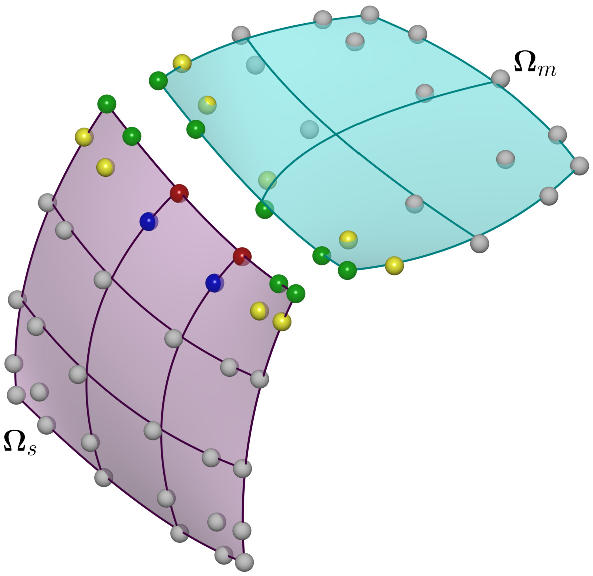
\includegraphics[width=.5\columnwidth]{control_points_classification}
	\caption{The classification of all basis functions for the two-patch non-conforming Kirchhoff-Love shell in Figure~\ref{fig:two_patch_shell_with_kink}. (For interpretation of colors in this figure, the reader is referred to the web version of this article.)}\label{fig:control_point_classification}
\end{figure}

We reorder the basis functions as well as the Lagrange multipliers by introducing two permutation matrices $\mathbf{P}_\text{c}$ and $\mathbf{P}_\text{r}$ (this step is not neccessary from the implementation point-of-view, but is helpful during the derivation, especially for multi-patch problems). We define the column-wise permutation matrix $\mathbf{P}_\text{c}$ as
\begin{equation}
	\begin{bmatrix}
		\mathbf{I}_\text{i}   \\
		\mathbf{I}_\text{ii}  \\
		\mathbf{I}_\text{iii} \\
		\mathbf{I}_\text{iv}  \\
		\mathbf{I}_\text{v}
	\end{bmatrix}=
	\mathbf{P}_\text{c}
	\begin{bmatrix}
		\mathbf{I}_s \\
		\mathbf{I}_m
	\end{bmatrix},
\end{equation}
where $\mathbf{I}_i$ is the vector form of the index set  $I_i$. We also define a row-wise permutation matrix $\mathbf{P}_\text{r}$ such that the permuted constraint matrix can be written in the partitioned form
\begin{equation}
	\mathbf{B}_\text{p}=\left[ \mathbf{P}_\text{r}\otimes\mathbf{I}_{3\times 3} \right]\mathbf{B}_\text{kl}\left[\mathbf{P}_\text{c}\otimes\mathbf{I}_{3\times 3}\right]^T=
	\begin{bmatrix}
		\mathbf{B}_1^1 & \mathbf{B}_1^2 & \mathbf{B}_1^3 & \mathbf{B}_1^4 & \mathbf{0} \\
		\mathbf{0}     & \mathbf{B}_2^2 & \mathbf{B}_2^3 & \mathbf{0}     & \mathbf{0}
	\end{bmatrix},
\end{equation}
where $\otimes$ is the tensor product operator, $\mathbf{I}_{3\times 3}$ is the ${3\times 3}$ identity matrix, $\mathbf{B}_1^1$ is the contribution of the first type of B-spline basis function in the discretization of $b_1$ and $\mathbf{B}_2^2$ is the contribution of the second type of B-spline basis function in the discretization of $b_0$. Under the row-wise permutation matrix $\mathbf{P}_\text{r}$, $\mathbf{B}_1^1$ and $\mathbf{B}_2^2$ become identity submatrices. Under a rank-preserving transformation $\mathbf{T}$ we can eliminate the submatrix $\mathbf{B}_1^2$ such that
\begin{equation}
	\sbox0{$\begin{matrix}\mathbf{B}_1^3-\mathbf{B}_1^2\mathbf{B}_2^3 & \mathbf{B}_1^4 & \mathbf{0} \\ \mathbf{B}_2^3 & \mathbf{0} & \mathbf{0}\end{matrix}$}
	\mathbf{T}\mathbf{B}_\text{p}=\left[
		\begin{array}{c:c}
			\makebox[\wd0/3]{\large $\mathbf{I}$} & \usebox{0} \\
		\end{array}
		\right].\label{eq:simple_form}
\end{equation}
We may now take
\begin{equation}
	\mathbf{B}^\perp_\text{p}=
	\left[\begin{array}{ccc}
			\mathbf{B}_1^2\mathbf{B}_2^3-\mathbf{B}_1^3 & -\mathbf{B}_1^4 & \mathbf{0}        \\
			-\mathbf{B}_2^3                             & \mathbf{0}      & \mathbf{0}        \\ \hdashline[2pt/2pt]
			\multicolumn{3}{c}{\multirow{3}{*}{\raisebox{0mm}{\scalebox{1.5}{$\mathbf{I}$}}}} \\
			                                            &                 &
		\end{array}\right].
\end{equation}
The vector basis of the null space of $\mathbf{B}_b$ can now be obtained from
\begin{equation}
	\mathbf{B}^\perp_\text{kl}=\left[\mathbf{P}_\text{c}\otimes\mathbf{I}_{3\times 3}\right]^T\mathbf{B}^\perp_\text{p}.\label{eq:permuted_back_nullspace}
\end{equation}
When the constraint is not homogeneous, i.e. $\mathbf{R}=\begin{bmatrix}
		\mathbf{0} & \mathbf{R}_{b_1}
	\end{bmatrix}^T\neq \mathbf{0}$, we have
\begin{equation}
	\mathbf{T}\mathbf{B}_\text{p}\left[\mathbf{P}_\text{c}\otimes\mathbf{I}_{3\times 3}\right]\mathbf{U}^\text{non} = \mathbf{T}\mathbf{R}_\text{p} = \mathbf{R}_\text{p},
\end{equation}
where $\mathbf{R}_\text{p}=\left[ \mathbf{P}_\text{r}\otimes\mathbf{I}_{3\times 3} \right]\mathbf{R}$. We can explicitly construct a particular solution from Equation~\eqref{eq:dual_particular_solution} as
\begin{equation}
	\mathbf{U}^\text{non} = \left[ \mathbf{P}_\text{r}\otimes\mathbf{I}_{3\times 3} \right]^T\mathbf{R}_\text{p} = \mathbf{R}.
\end{equation}

\section{Numerical results}\label{sec:numerical}

In this section, the performance of the proposed Kirchhoff-Love shell coupling formulation as well as the enriched \Bezier dual basis are illustrated by several challenging benchmark examples, including both linear and non-linear problems. Results computed using the $i^\text{th}$ order global dual basis are labeled $G-Q_i$. Results computed using the $i^\text{th}$ order enriched \Bezier dual basis are labeled $B-Q_i$. Note that the $i^\text{th}$ order enriched \Bezier dual basis is constructed by reproducing polynomials of degree $i-2$.

\subsection{Linear problems}

In this subsection, we consider the performance of the proposed patch coupling formulation for the linearized Kirchhoff-Love shell model. The first example is a simply supported plate under sinusoidal load, where results are compared with the analytical solution. The second example is the Scordelis-Lo roof problem. The convergence behavior is tested against a numerical solution from a very fine mesh. In the third example, we consider a hemisphere shell subjected to two opposite point loads. Two different parameterizations are considered. All problems in this subsection are solved by the conjugate gradient iterative solver in Eigen library~\cite{eigenweb}.

\subsubsection{Simply supported plate under sinusoidal load}
\begin{figure}[h]
	\center
	\begin{subfigure}[t]{.45\linewidth}
		\center
		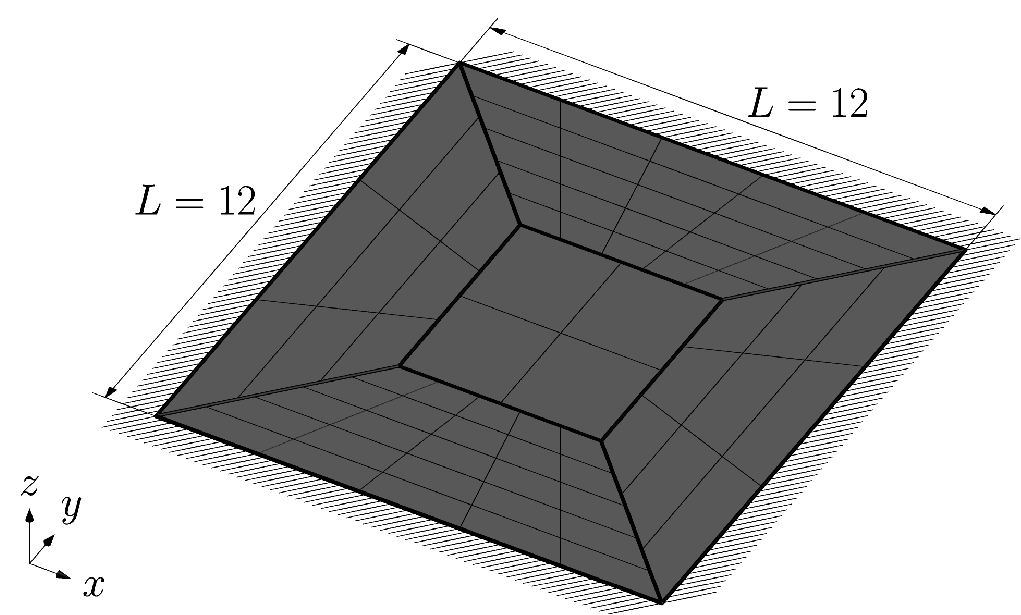
\includegraphics[scale=.36]{plate_config1}
		\caption{Non-matching parameterized non-conforming three-patch mesh}
	\end{subfigure}
	\begin{subfigure}[t]{.45\linewidth}
		\center
		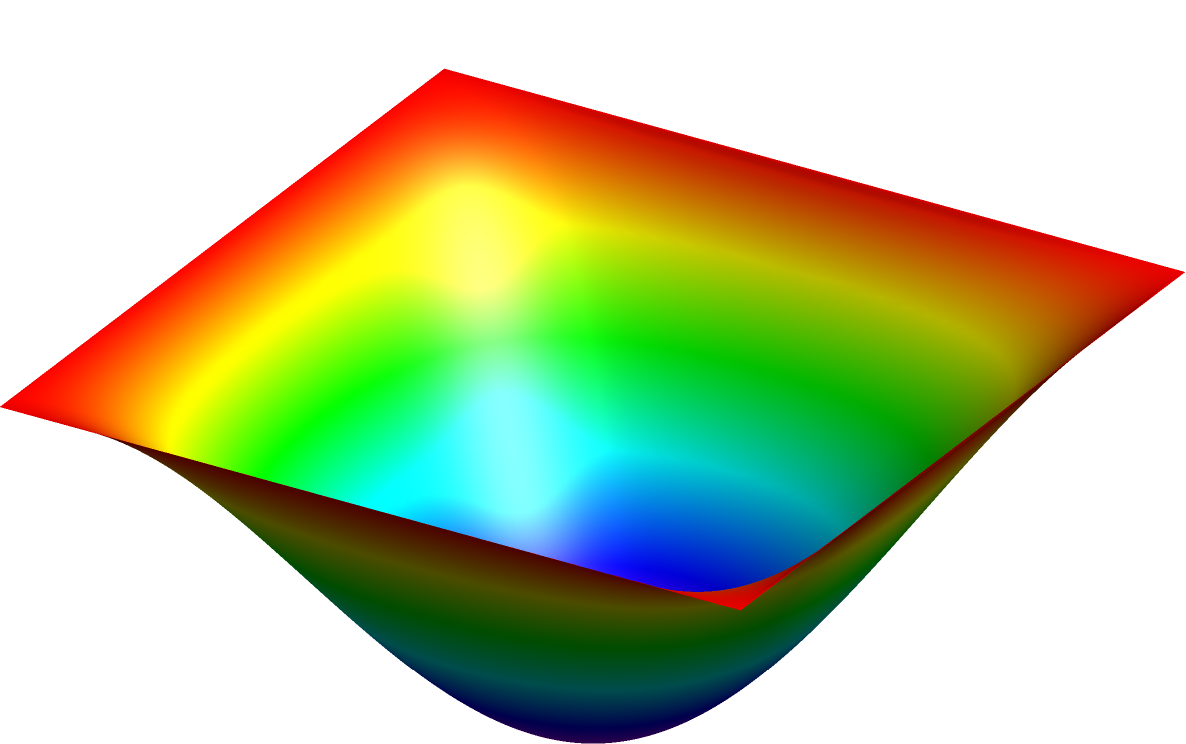
\includegraphics[scale=.28]{plate_solution-plot}
		\caption{The reference solution}
	\end{subfigure}
	\caption{The decomposition and parameterization of the domain $\left[0, 12\right] \times \left[0, 12\right]$ and the refernce solution that satisfies $u=0$ on $\partial\Omega$.}\label{fig:kirchhoff_plate_mesh}
\end{figure}
In the first example, we study a plate of size $L\times L = 12\times 12$, thickness $t=0.375$, Young's modulus $E=4.8\times 10^5$, Poisson's ratio $\nu = 0.38$ and subjected to a sinusoidal pressure $p(x, y) = \sin(\pi \frac{x}{L})\sin(\pi \frac{y}{L})$ (in $-z$ direction). The analytical solution of the vertical displacement is given by~\cite{timoshenko1959theory} (see Figure~\ref{fig:kirchhoff_plate_mesh})
\begin{equation}
	w(x, y) = -\frac{L^4}{4D\pi^4}\sin(\frac{\pi x}{L}) \sin(\frac{\pi y}{L}),
\end{equation}
where $D = \frac{Et^3}{12(1-\nu^2)}$ is the flexural rigidity of the plate. The computational domain is decomposed into five non-conformingly coupled patches as shown in Figure~\ref{fig:kirchhoff_plate_mesh}. The simply supported boundary condition is applied by setting $\mathbf{u}=0$ on the boundary.\par
\begin{figure}[h]
	\center
	\captionsetup[subfigure]{labelformat=empty}
	\begin{subfigure}{.47\linewidth}
		\center
		\includestandalone[scale=.75]{plate_L2}
	\end{subfigure}\hfil
	\begin{subfigure}{.47\linewidth}
		\center
		\includestandalone[scale=.75]{plate_Mx}
	\end{subfigure}
	\begin{subfigure}{.47\linewidth}
		\center
		\includestandalone[scale=.75]{plate_Mxy}
	\end{subfigure}
	\caption{Convergence plots for the simply supported plate under sinusoidal pressure load. Upper left: error of $w$ measured in $L^2$ norm. Upper right: error of $M_{xx}$ measured in $L^2$ norm. Bottom: error of $M_{xy}$ measured in $L^2$ norm.}\label{fig:convergence_square_plate}
\end{figure}
Figure~\ref{fig:convergence_square_plate} shows the convergence of the approximated vertical displacement $w^h$, bending moment $M^h_{xx}$ and $M^h_{xy}$ to the analytical solution as the mesh is refined. As expected, both the enriched \Bezier dual basis and the global dual basis yield optimal results for all polynomial orders in all three measures. For the displacement error, there is no visible difference between the enriched \Bezier dual basis and the global dual basis in all tested polynomial orders. However, compared to the global dual basis, the enriched \Bezier dual basis introduces slightly higher errors in both $M_{xx}$ and $M_{xy}$ errors for $p = 3,4$, though the convergence remains optimal. \par

Contour plots of $\text{err} = u_z^h-u_z$, $\text{err} = M_{xx}^h-M_{xx}$ and $\text{err} = M_{xy}^h-M_{xy}$ for cubic splines are given in Figure~\ref{fig:contour_d_mxx_mxy_plate}. The error level for two types of dual basis are very similar in all three error measures. For the enriched \Bezier dual basis case, error spikes are formed along intersections and highest error spikes are observed at vertices for $M_{xx}$ and $M_{xy}$. The global dual basis, on the other hand, seems to yield more evenly distributed errors.

\begin{figure}[h]
	\center
	\captionsetup[subfigure]{labelformat=empty}
	\begin{subfigure}[t]{.45\linewidth}
		\center
		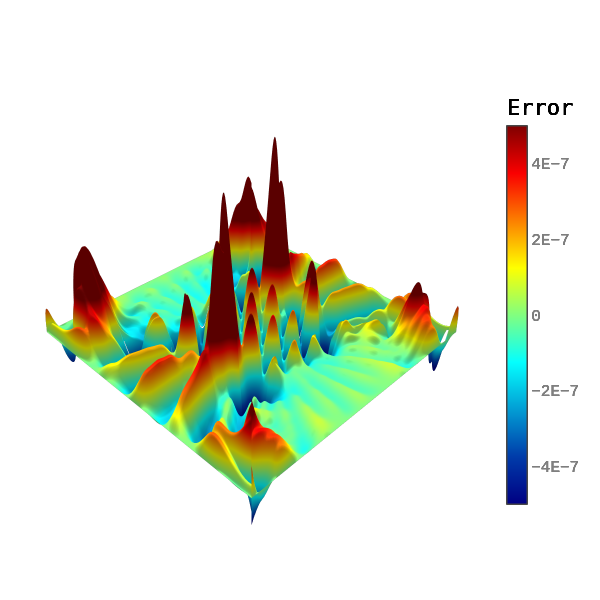
\includegraphics[scale=.3,trim={0cm 1.5cm 0cm 1.5cm},clip]{e_d}
		\caption{$B-Q_3$ $\quad \text{err} = u_z^h-u_z$}
	\end{subfigure}
	\begin{subfigure}[t]{.45\linewidth}
		\center
		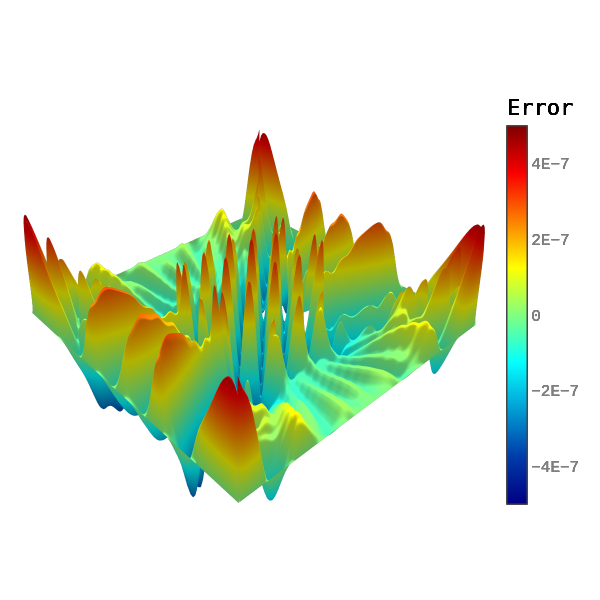
\includegraphics[scale=.3,trim={0cm 1.5cm 0cm 1.5cm},clip]{g_d}
		\caption{$G-Q_3$ $\quad \text{err} = u_z^h-u_z$}
	\end{subfigure}\\
	\begin{subfigure}[t]{.45\linewidth}
		\center
		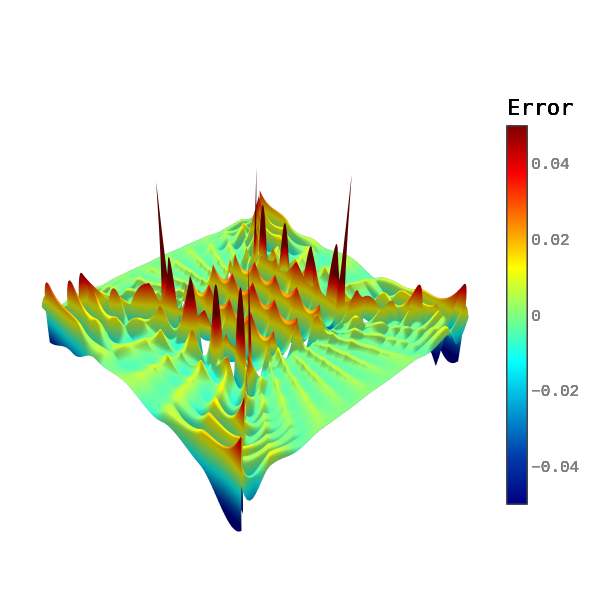
\includegraphics[scale=.3,trim={0cm 1.5cm 0cm 1.5cm},clip]{e_Mxx}
		\caption{$B-Q_3$ $\quad \text{err} = M_{xx}^h-M_{xx}$}
	\end{subfigure}
	\begin{subfigure}[t]{.45\linewidth}
		\center
		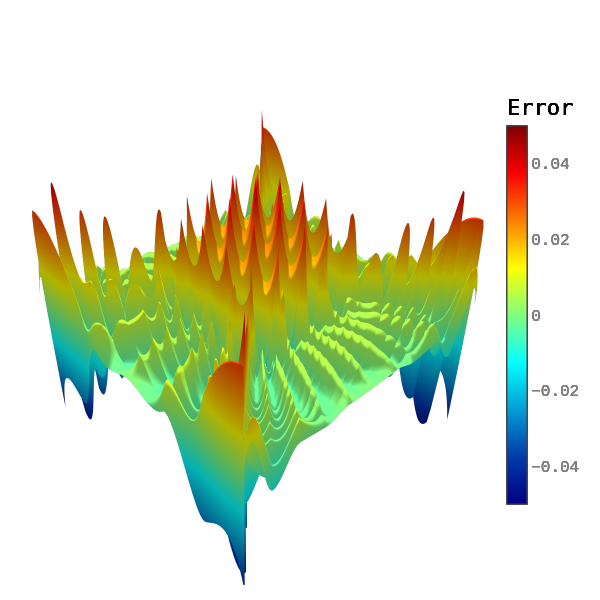
\includegraphics[scale=.3,trim={0cm 1.5cm 0cm 1.5cm},clip]{g_Mxx}
		\caption{$G-Q_3$ $\quad \text{err} = M_{xx}^h-M_{xx}$}
	\end{subfigure}\\
	\begin{subfigure}[t]{.45\linewidth}
		\center
		\includegraphics[scale=.3,trim={0cm 1.5cm 0cm 1.5cm},clip]{e_Mxy}
		\caption{$B-Q_3$ $\quad \text{err} = M_{xy}^h-M_{xy}$}
	\end{subfigure}
	\begin{subfigure}[t]{.45\linewidth}
		\center
		\includegraphics[scale=.3,trim={0cm 1.5cm 0cm 1.5cm},clip]{g_Mxy}
		\caption{$G-Q_3$ $\quad \text{err} = M_{xy}^h-M_{xy}$}
	\end{subfigure}
	\caption{Contour plots of $\text{err} = u_z^h-u_z$, $\text{err} =  M_{xx}^h- M_{xx}$ and $\text{err} =  M_{xy}^h- M_{xy}$ for the simply supported plate under sinusoidal load ($p=3$, and the mesh is obtained after one refinement). }\label{fig:contour_d_mxx_mxy_plate}
\end{figure}
\FloatBarrier
\subsubsection{Scordelis-Lo roof problem}

We then consider the Scordelis-Lo roof benchmark problem. The Scordelis-Lo roof problem is a membrane stress dominated static shell problem and named after the authors who first reported it~\cite{scordelis1964computer}. In this problem, a cylindrical shell roof (Young's modulus $E=432\text{MPa}$, Poisson's ratio $\nu = 0$, thickness $t = 0.25\text{m}$.), under the distributed gravity load ($f = 90\text{N}/\text{m}^2$), is supported by rigid diaphragms on both curved edges (i.e. $u_{x}=u_z=0$), while the straight edges are free to move, as depicted in Figure.~\ref{fig:scordelis-lo}. To improve the robustness, the displacement in $y$ direction of one DOF on the diaphragms supported edges is fixed. The vertical displacement at the midpoint of the straight edges is considered as the reference (with the given value $u_z=-0.300592457\text{m}$~\cite{coox2017flexible}).\par

\begin{figure}[h]
	\centering
	\captionsetup[subfigure]{font = footnotesize}
	\begin{subfigure}[b]{.33\textwidth}
		\centering
		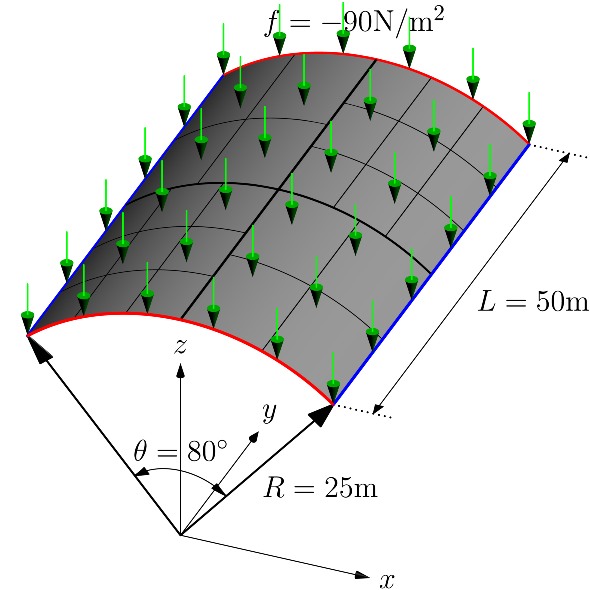
\includegraphics[width = \textwidth]{roof_config1}
		\caption{}\label{fig:scordelis-lo}
	\end{subfigure}\hfil
	\begin{subfigure}[b]{.66\textwidth}
		\centering
		
\includegraphics[width = .48\textwidth]{roof_c0_result}
		
\includegraphics[width = .48\textwidth]{roof_c1_result}
		\caption{}\label{fig:scordelis_deform}
	\end{subfigure}
	% \begin{subfigure}[b]{.48\textwidth}
	% 	\centering
	% 	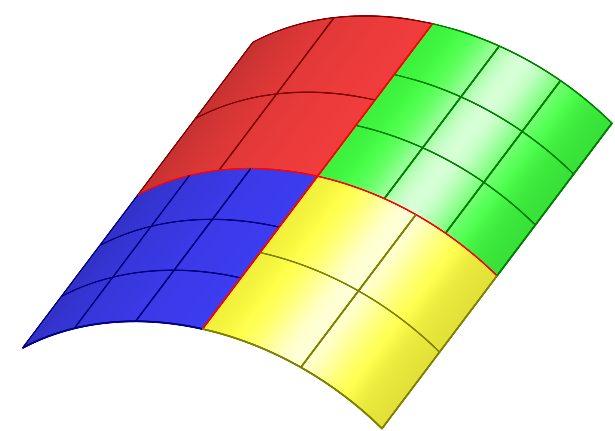
\includegraphics[width = \textwidth]{roof_decompose}
	% 	\vspace{.5cm}
	% 	\caption{Non-conforming four patch mesh with the intersections denoted by red lines.}\label{fig:scordelis-lo-decompose}
	% \end{subfigure}
	\caption{The Scordelis-Lo roof problem: (a) Geometry, parameterization and boundary conditions. Note that the blue edges are free, while the red edges are fixed in $x$ and $z$ directions. (b) Deformed Scordelis-Lo roof (scaling factor of 20 is applied to the displacement). Left: Only the $C^0$ continuity constraint is applied. After deformation, kinks are formed on all intersections. Right: The $C^1$ continuity constraint is also applied. The deformed surface is as smooth as a single patch.}
\end{figure}

The roof structure is decomposed into four patches, which are discretized non-conformingly as shown in Fig.~\ref{fig:scordelis-lo}. Fig.~\ref{fig:scordelis_deform} demonstrates the effect of the proposed constraint. As can be seen, with only $C^0$ continuity constraint enforced, althought the deformed surface remains continuous, all intersections fail to transfer the bending moments from one patch to another. Hence, connections act like hinges and kinks are formed along all intersections. By enforcing the additional constraint, the smoothness of the roof structure is preserved, even though the mesh is non-conformingly discretized. \par

% \begin{figure}[h]
% 	\centering
% 	\captionsetup[subfigure]{font = footnotesize}
% 	\begin{subfigure}[b]{.49\textwidth}
% 		\centering
% 		
\includegraphics[width = \textwidth]{roof_c0_result}
% 		\caption{}
% 	\end{subfigure}
% 	\begin{subfigure}[b]{.49\textwidth}
% 		\centering
% 		
\includegraphics[width = \textwidth]{roof_c1_result}
% 		\caption{}
% 	\end{subfigure}
% 	\caption{Deformed Scordelis-Lo roof (scaling factor of 20 is applied to the displacement): (a) Only the $C^0$ continuity constraint is applied. After deformation, kinks are formed on all intersections. (b) The $C^1$ continuity constraint is also applied. The deformed surface is as smooth as a single patch.}\label{fig:scordelis_deform}
% \end{figure}

The sparsity patterns for the stiffness matrices corresponding to the coupled problem using the global dual basis, and the coupled problem using the enriched \Bezier dual basis are shown in Figure~\ref{fig:scordelis-lo-sparsity}. Note that the matrix constructed using the enriched \Bezier dual basis is much sparser then the matrix constructed using the global dual basis.\par

\begin{figure}[h]
	\centering
	\captionsetup[subfigure]{font = footnotesize}
	\begin{subfigure}[b]{.48\textwidth}
		\centering
		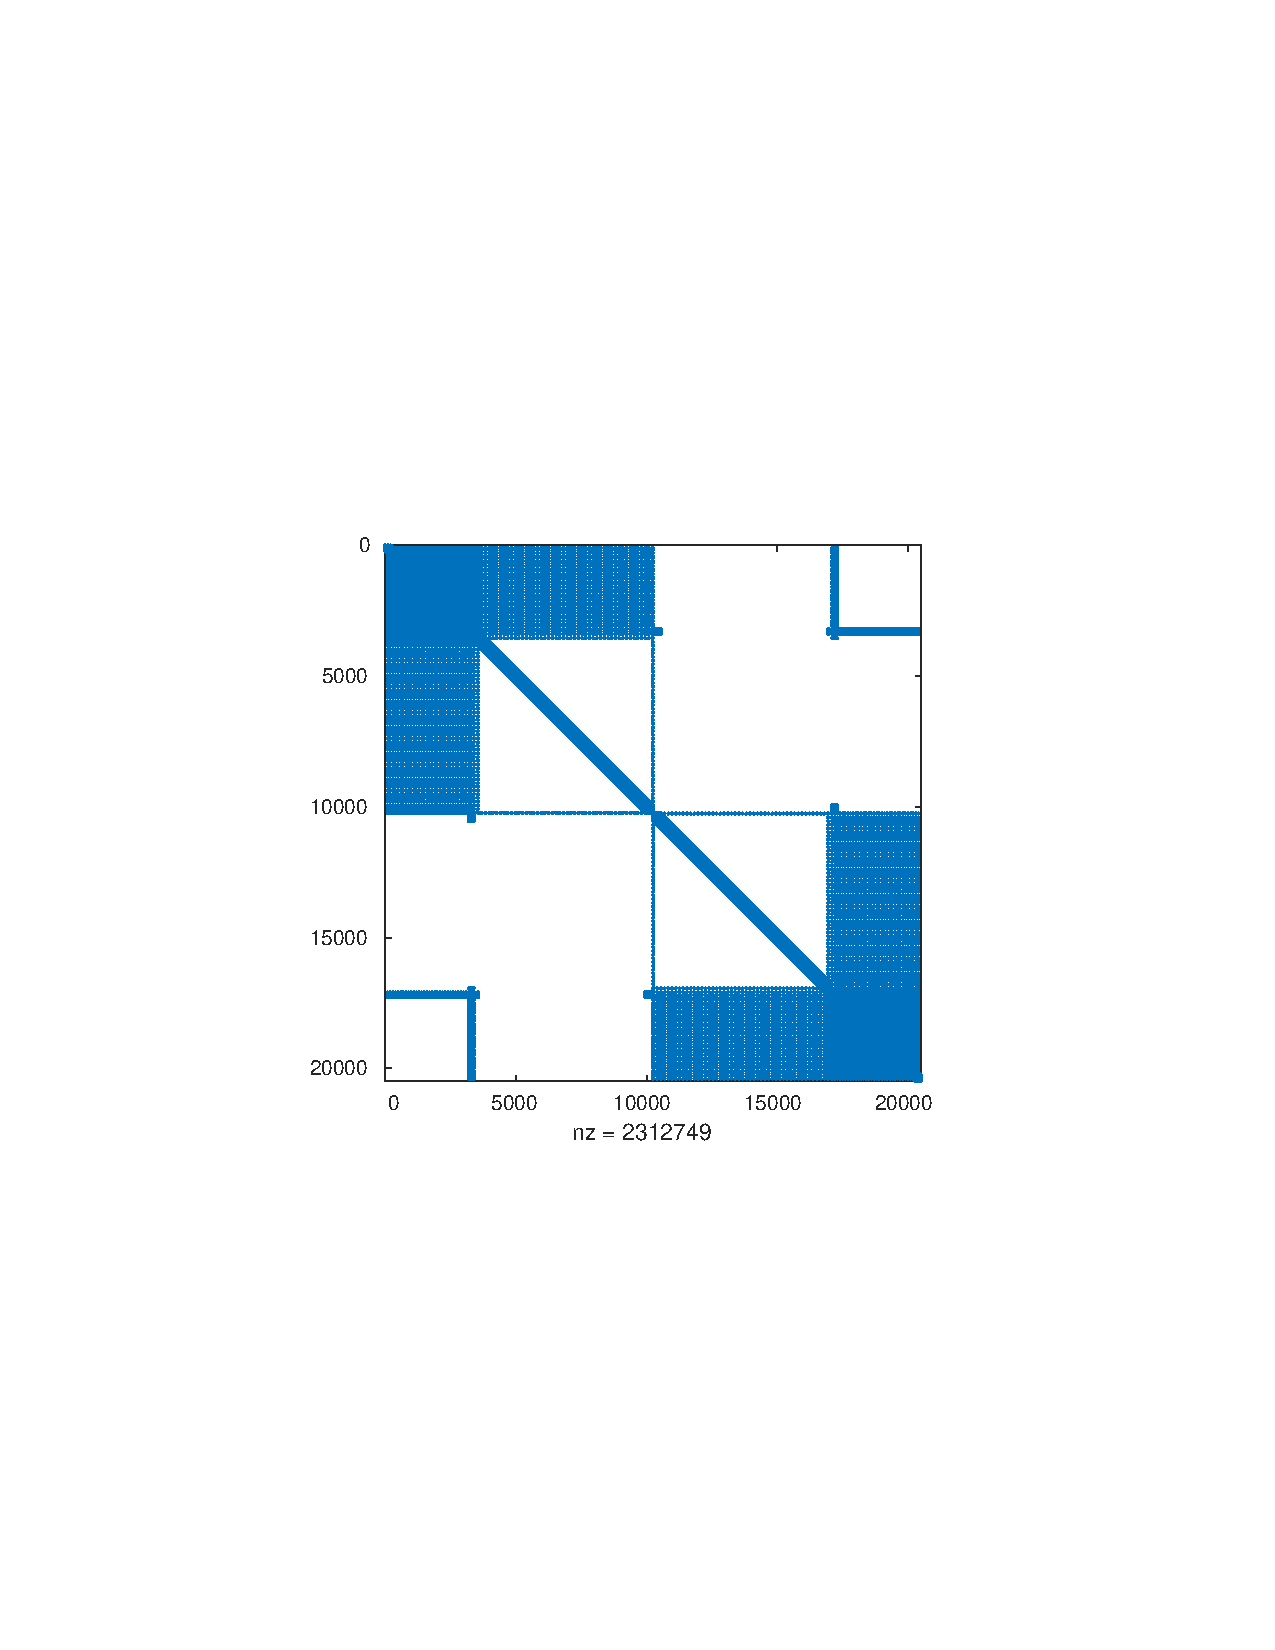
\includegraphics[clip, trim=5cm 8.5cm 5cm 9cm, width = .9\textwidth]{global_sparsity}
		\caption{}
	\end{subfigure}\hfil
	\begin{subfigure}[b]{.48\textwidth}
		\centering
		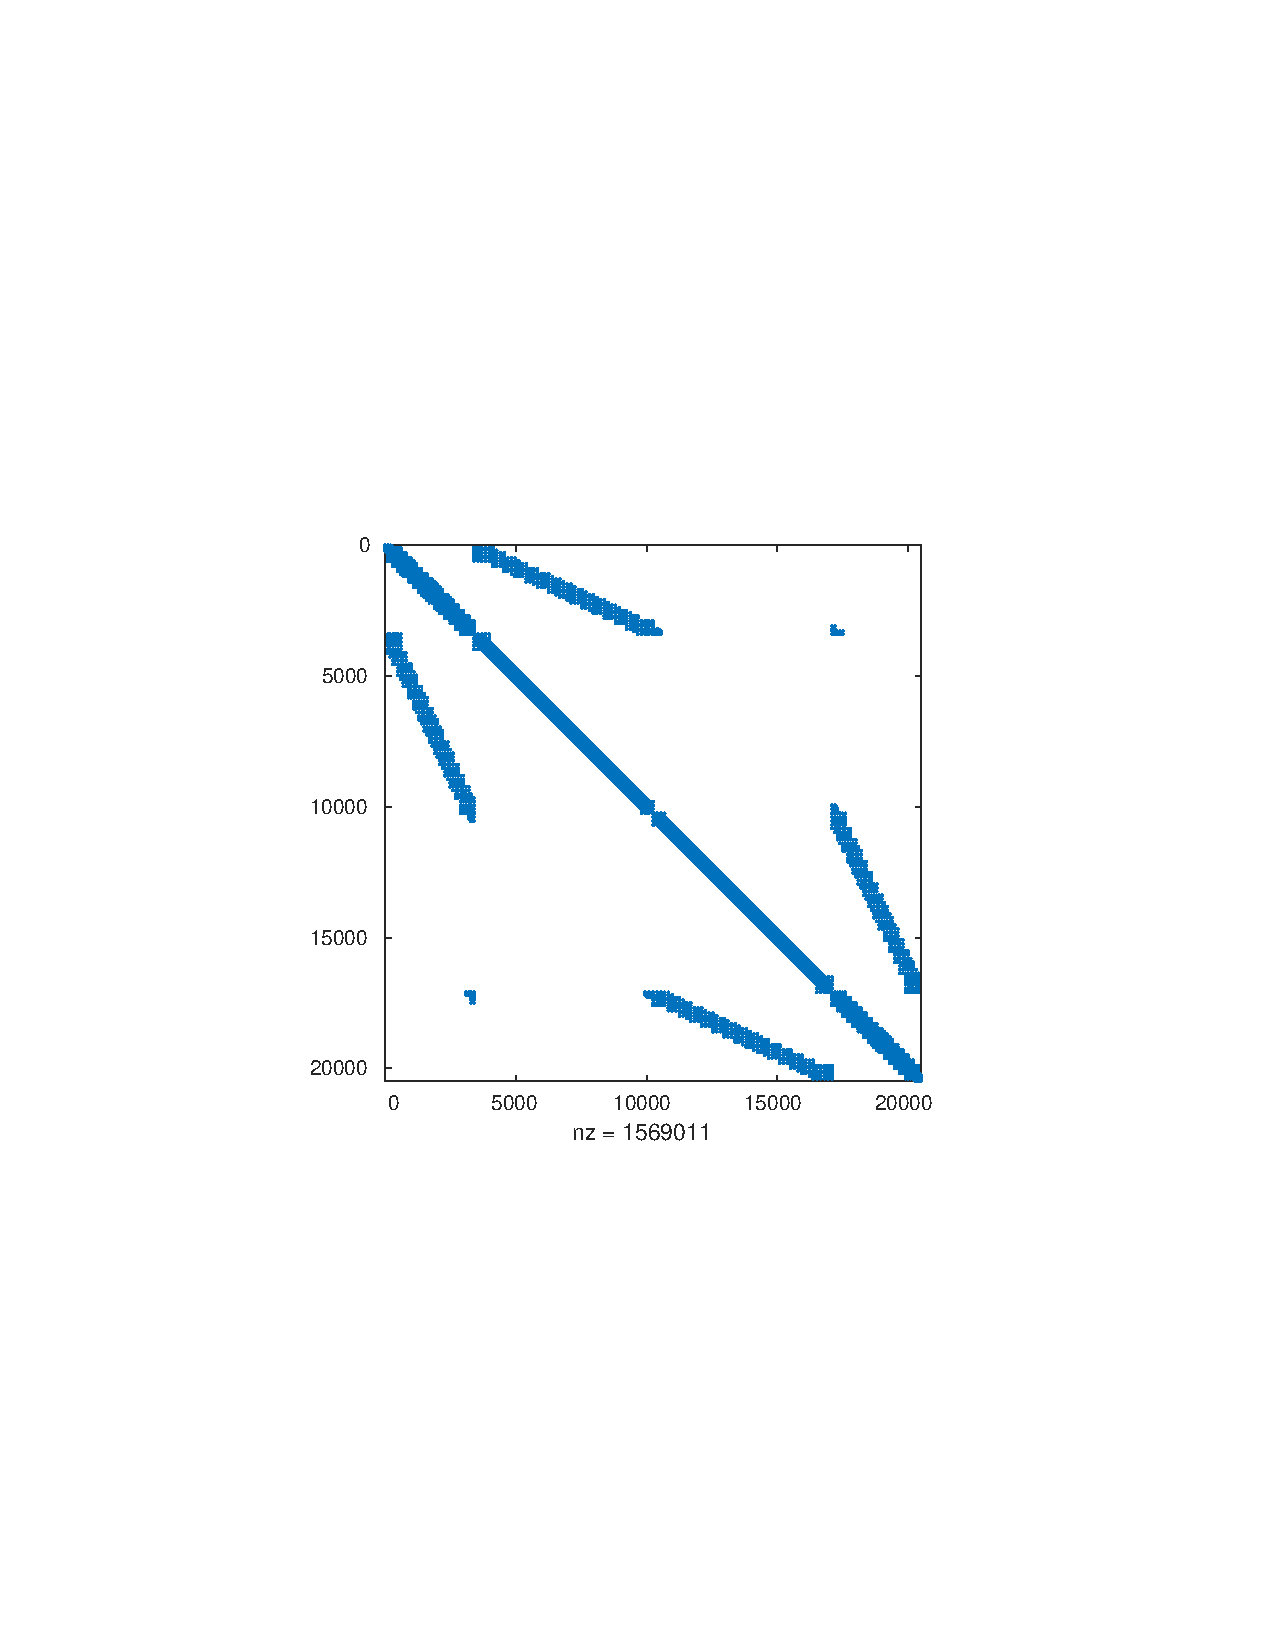
\includegraphics[clip, trim=5cm 8.5cm 5cm 9cm, width = .9\textwidth]{enriched_sparsity}
		\caption{}
	\end{subfigure}
	\caption{Stiffness matrix sparsity patterns for (a) the coupled linear system using the global dual basis, and (b) the coupled linear system using the enriched \Bezier dual basis for the Scordelis-Lo roof problem. The stiffness matrices are computed from the four-patch domain in Figure~\ref{fig:scordelis-lo} after $4$ levels of refinement.}\label{fig:scordelis-lo-sparsity}
\end{figure}

Fig.~\ref{fig:scordelis_displacement} shows the vertical displacement of the midpoint of the free edge for different polynomial degrees. Converged results are obtained by both the global dual basis and the enriched \Bezier dual basis for all polynomial orders. For quartic basis functions, the relative error is reduced to $0.1\%$ with only one refinement for both dual basis. The accuracy of the four-patch configurations is very similar to the single patch one. To better study the performance of the proposed coupling formulation, we compare the displacement field of the four-patch mesh to a reference solution obtained from a very fine single patch mesh, as shown in Figure~\ref{fig:convergence_scordelis}. Optimal convergence rates are attained for all polynomial orders. The convergence plots of the enriched \Bezier dual basis is indistinguishable to that of the global dual basis.

\begin{figure}[h]
	\centering
	\captionsetup[subfigure]{font = footnotesize}
	\begin{subfigure}[b]{.32\textwidth}
		\centering
		\includestandalone[scale=.8]{Scordelis-Lo-p=2}
		\caption{}
	\end{subfigure}
	\begin{subfigure}[b]{.32\textwidth}
		\centering
		\includestandalone[scale=.8]{Scordelis-Lo-p=3}
		\caption{}
	\end{subfigure}
	\begin{subfigure}[b]{.32\textwidth}
		\centering
		\includestandalone[scale=.8]{Scordelis-Lo-p=4}
		\caption{}
	\end{subfigure}
	\caption{Scordelis-Lo roof problem: a comparison of the vertical displacement at the midpoint of the free edge for different dual basis functions and degrees.}\label{fig:scordelis_displacement}
\end{figure}

\begin{figure}[h]
	\center
	\includestandalone[scale=1]{Scordelis-Lo_convergence}
	\caption{The convergence plot for the Scordelis-Lo roof problem.}\label{fig:convergence_scordelis}
\end{figure}
\FloatBarrier
\subsubsection{Pinched hemispherical shell problem}

\begin{figure}[h]
	\centering
	\captionsetup[subfigure]{font = footnotesize}
	\begin{subfigure}[b]{.48\textwidth}
		\centering
		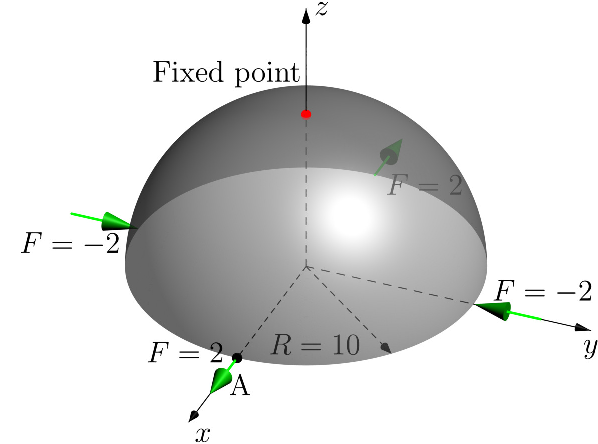
\includegraphics[width = \textwidth]{hemisphere_config}
		\caption{Geometry and boundary conditions of the problem. The red point is fixed from moving and rotating.}\label{fig:hemisphere-config}
	\end{subfigure}\hfil
	\begin{subfigure}[b]{.48\textwidth}
		\centering
		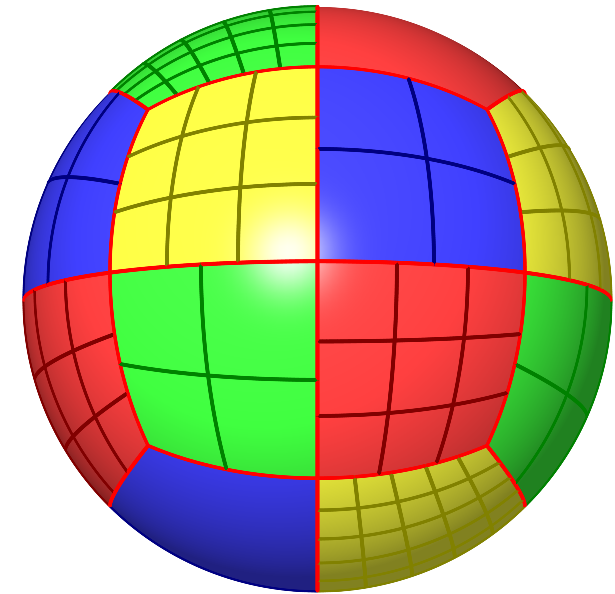
\includegraphics[width = .7\textwidth]{hemisphere_decompose}
		\caption{Non-conforming twelve patch mesh with the intersections denoted by the red lines.}\label{fig:hemisphere_decompose-2}
	\end{subfigure}
	\caption{The geometry and mesh setup of the pinched hemisphere shell problem.}\label{fig:hemisphere}
\end{figure}

In this example, we consider a hemispherical shell pinched at the top and subjected to four radial point loads (see Fig.~\ref{fig:hemisphere-config}). The bottom circumferential edge of the hemisphere is free. The thickness of the shell is $t = 0.04$ and the material properties are $E = 6.825\times{}10^7$ and $\nu = 0.3$. The hemispherical is decomposed into twelve patches as shown in Figure~\ref{fig:hemisphere_decompose-2}. Note that the twelve-patch parameterization is degeneracy-free. The radial displacement at point A is considered as the benchmark quantity and a reference value is given as $u_x = 0.0924$~\cite{kiendl2009isogeometric}.\par

The convergence of the proposed formulation is plotted in Figure~\ref{fig:hemisphere_result}. Convergence is observed for both types of dual basis functions. It seems that, as the mesh is refined, the enriched \Bezier dual basis provides results that are closer to the reference solution.  
\begin{figure}[h]
	\center
	\includestandalone[scale = 1]{twelve-patch-hemisphere}
	\caption{ Pinched hemispherical shell problem: acomparison of the radial displacement at point A for different dual basis functions and degrees}
	\label{fig:hemisphere_result}
\end{figure}
\FloatBarrier
\subsubsection{T-beam}

Shell structrues with kinks and sharp folds are widely applied in engineering practice. In this example, we verify the performance of the proposed coupling formulation in preserving the coupling angle between patches during deformation. A T-beam (see Herrema et al.~\cite{herrema2019penalty}) with a thickness of $t=0.1$ in Figure~\ref{fig:T-beam-config} is modelled by three cubic B-spline patches joined at a common edge, where the flange is formed by $14\times 4$ and $ 16\times 4$ B-spline patches and the web is formed by a $12\times 4$ B-spline patch. The T-beam is pinned (i.e. $\mathbf{u}=0$) on one side and deflected under a point load of $F = 10$ at one corner of the flange in the $-z$ direction (see Figure~\ref{fig:T-beam-config}). The deformed configuration is shown in Figure~\ref{fig:T-beam-deform}, a maximum displacement magnitude of $\max(\vert \mathbf{u} \vert)=0.0589$ is observed at the bottom tip of the web, which agrees with the result in~\cite{herrema2019penalty}. \par

\begin{figure}[h]
	\center
	\begin{subfigure}[b]{0.43\textwidth}
		\centering
		% 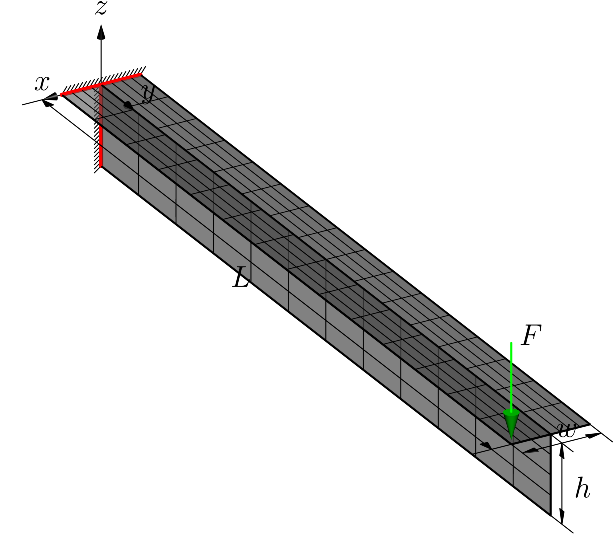
\includegraphics[width = \textwidth]{T-beam-config}
		\begin{tikzpicture}
			\node[inner sep=0pt] at (0,0)
			{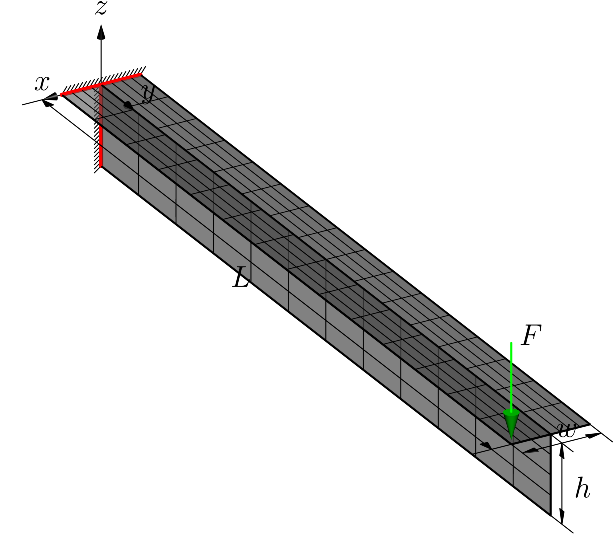
\includegraphics[width=\textwidth]{T-beam-config}};
			\node[draw,align=left] at (2.2,1) {$L=20$\\$w=2$\\$h=2$};
		\end{tikzpicture}
		\caption{}\label{fig:T-beam-config}
	\end{subfigure}
	\begin{subfigure}[b]{0.54\textwidth}
		\centering
		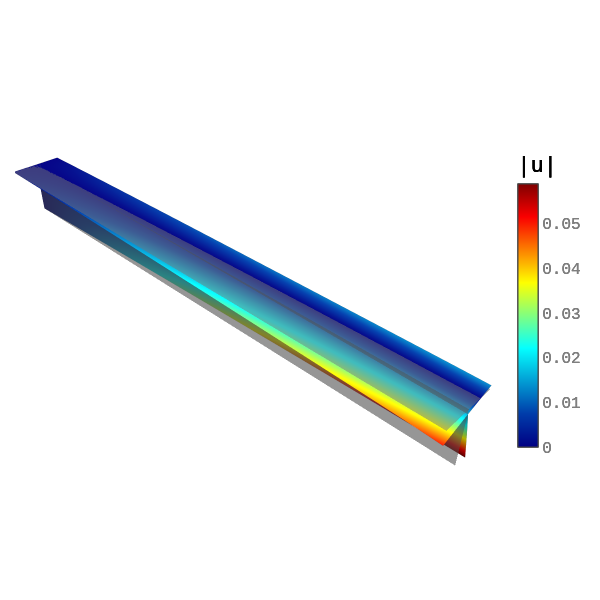
\includegraphics[width = \textwidth,trim={0cm 4cm 0cm 1cm},clip]{t-beam_deform}
		\caption{}\label{fig:T-beam-deform}
	\end{subfigure}
	\caption{T-beam prolem: (a) Geometry, parameterization and boundary conditions of the problem. Note that red edges are pinned ends (i.e. $\mathbf{u}=0$). (b) Deformed configuration with a scale factor of $10$. }
	\label{fig:T-beam}
\end{figure}


Figure~\ref{fig:T-beam_angle} shows the relative error between the deformed coupling angle and the original $90^\circ$ coupling angle between the web and flange for the mesh in Figure~\ref{fig:T-beam-config} (coarse) and the one after one refinement (fine). In the region $y\in\left[0, 10\right]$ for the coarse mesh and $y\in\left[0, 14\right]$ for the fine mensh, we observe a relative error close to zero. Oscillations are observed at the free end of the intersection for all tested cases. We attribute this phenomenon to the dimonsion of the discretized Lagrange multiplier spaces. Lagrange multiplier with codimension four of the trace space renders all twelve control points at the free end of the intersection become master nodes so that constraints at this region could not transfer stresses from one patch to the other. However, a $h-$refinement does reduce the error magnitude as well as the size of the oscillation region. Owing to the compact supports, the oscillation region of the result from the enriched \Bezier dual basis is smaller than the result from the global dual basis for both coarse and fine meshes. \par

\begin{figure}[h]
	\center
	\begin{subfigure}[b]{0.47\textwidth}
		\centering
		\includestandalone[scale=.8]{T-beam_angle_coarse}
		\caption{}
	\end{subfigure}
	\begin{subfigure}[b]{0.47\textwidth}
		\centering
		\includestandalone[scale=.8]{T-beam_angle_fine}
		\caption{}
	\end{subfigure}
	\caption{Relative error of angle between the flange and web along the intersection for (a) a coarse mesh, (b) a fine mesh. }
	\label{fig:T-beam_angle}
\end{figure}
\FloatBarrier

\subsection{Nonlinear problems}

The proposed formulation has demonstrated its accuracy in linear analysis. In the following, the robustness of the proposed formulation will be verified by several challenging nonlinear benchmark problems. From our observations, the presence of the geometric stiffness matrix significantly influences the convergence of the conjugate gradient solver. For the sake of robustness, all problems in this subsection are solved by SparseLU module in Eigen library~\cite{eigenweb}.

\subsubsection{Cantilever subjected to an end shear force}

The first nonlinear problem to be studied is a cantilever subjected to an end shear force (see Figure~\ref{fig:cantilever_config}). The length, width and thickness of the cantilever are $L = 10$, $b = 1$ and $t = 0.1$, respectively. The material parameters are: Young's modulus $E = 1.2\times 10^6$ and Poisson's ratio $\nu = 0$. The left boundary is clamped ($\mathbf{u}=\frac{\partial \mathbf{u}}{\partial x}=0$) while the right boundary is subjected to a uniformly distributed traction load in the $z$-direction with the maximum load of $f=4$ and the incremental load of $\Delta f = 0.4$. The cantilever is decomposed into three patches, which are discretized by $9\times 3$, $5\times 2$ and $3\times 3$ B-spline elements, respectively (see Figure~\ref{fig:cantilever_mesh}). A fine mesh obtained by a uniform refinement of the mesh in Figure~\ref{fig:cantilever_mesh} is also considered in this research. The deformed cantilever is demonstrated in Figure~\ref{fig:cantilever_deform}.
% \begin{figure}[h]
% 	\center
% 	\begin{subfigure}[b]{\textwidth}
% 		\centering
% 		\begin{tikzpicture}
% 			\node[inner sep=0pt] at (0,0)
% 			{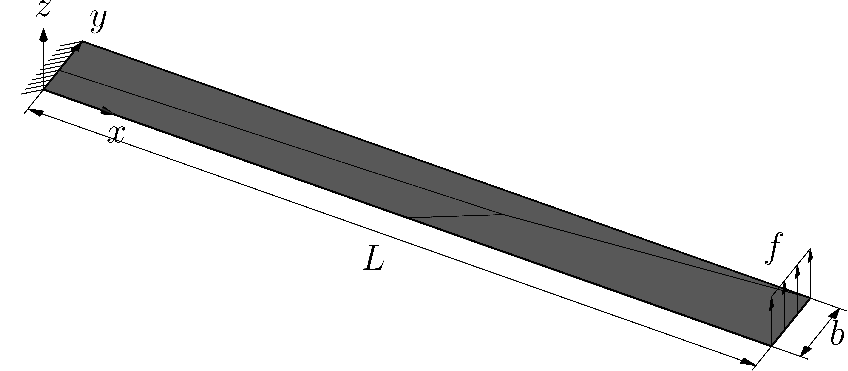
\includegraphics[width=.7\textwidth]{pure_shear_shell_config}};
% 			% \node[draw,align=left] at (7.2,0) {$E=1.2\times 10^6$\\$L=10$\\$\nu=0$\\$b=1$\\$f_\text{max}=4(\text{force/length})$\\$t=0.1$};
% 		\end{tikzpicture}
% 		% 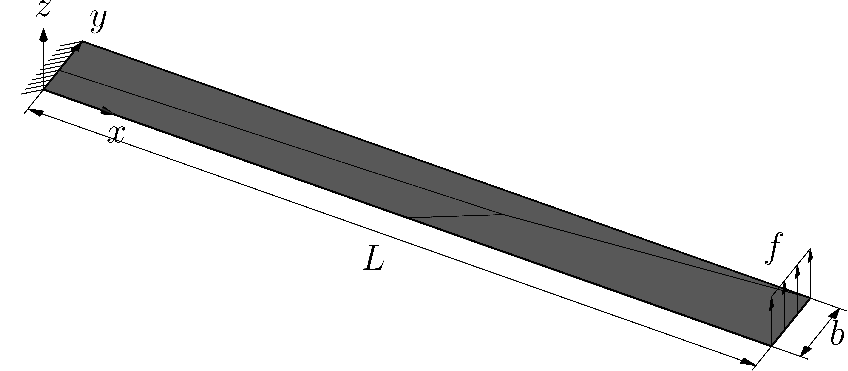
\includegraphics[scale=1]{pure_shear_shell_config}
% 		\caption{}\label{fig:cantilever_config}
% 	\end{subfigure}
% 	\\\hspace{1em}
% 	\begin{subfigure}[b]{\textwidth}
% 		\centering
% 		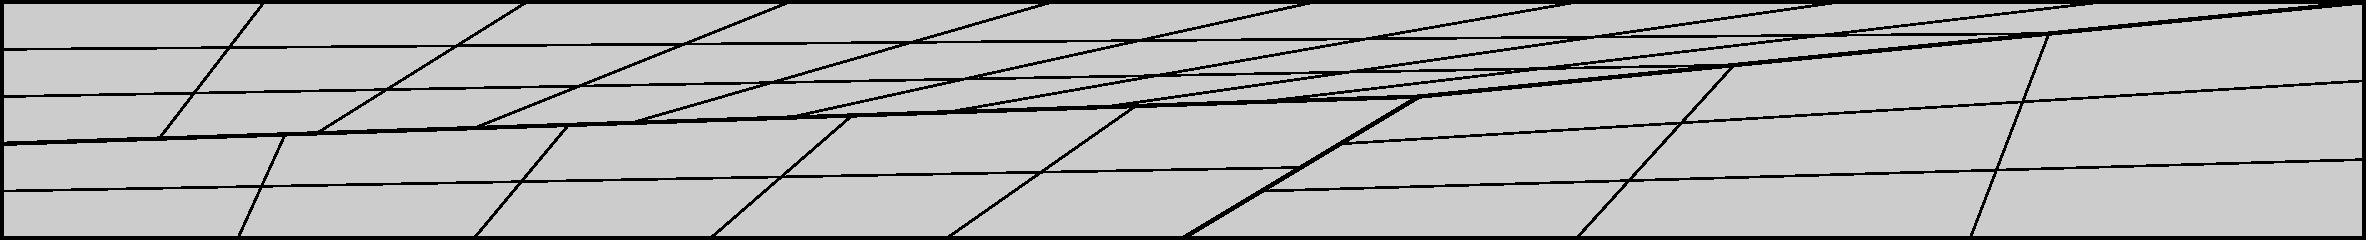
\includegraphics[scale=.35]{pure_shear_shell_mesh}
% 		\caption{}\label{fig:cantilever_mesh}
% 	\end{subfigure}
% 	\\\hspace{1em}
% 	\begin{subfigure}[b]{\textwidth}
% 		\centering
% 		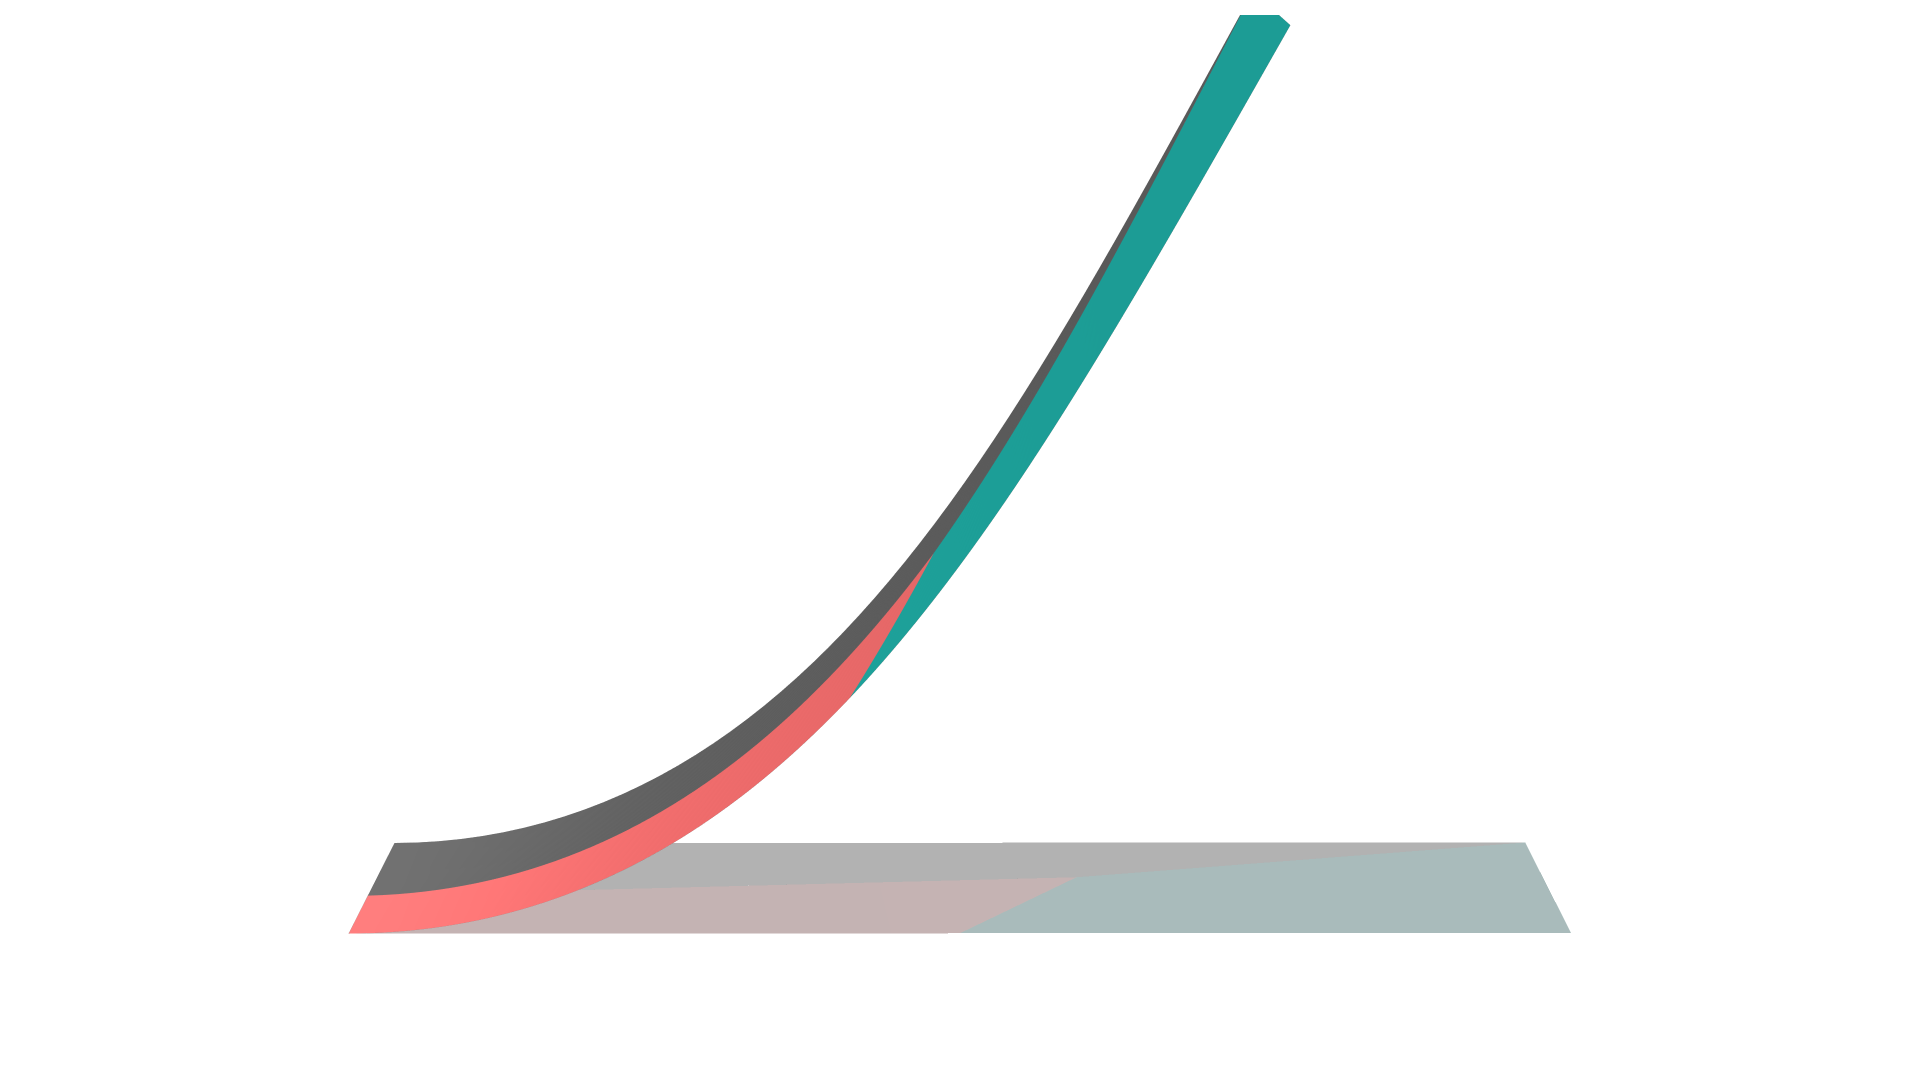
\includegraphics[scale=.2,trim={2cm 4cm 2cm 1cm},clip]{pure_shear_shell_deformed}
% 		\caption{}\label{fig:cantilever_deform}
% 	\end{subfigure}
% 	\caption{A cantilever subjected to an end shear force: (a) the problem description, (b) the three-patch non-matching discretization and (c) the initial and deformed configurations. }
% \end{figure}
\begin{figure}[h]
	\begin{tabular}[b]{cc}
		\begin{tabular}[b]{c}
			\begin{subfigure}[b]{0.48\columnwidth}
				\centering
				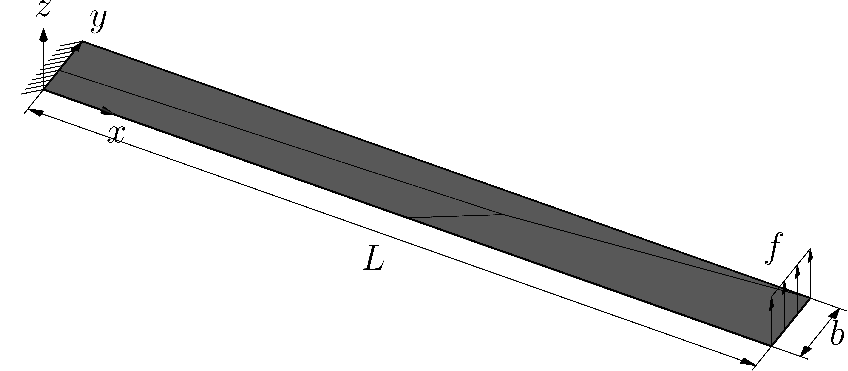
\includegraphics[width=\textwidth]{pure_shear_shell_config}
				\caption{}
				\label{fig:cantilever_config}
			\end{subfigure} \\
			\begin{subfigure}[b]{0.48\columnwidth}
				\centering
				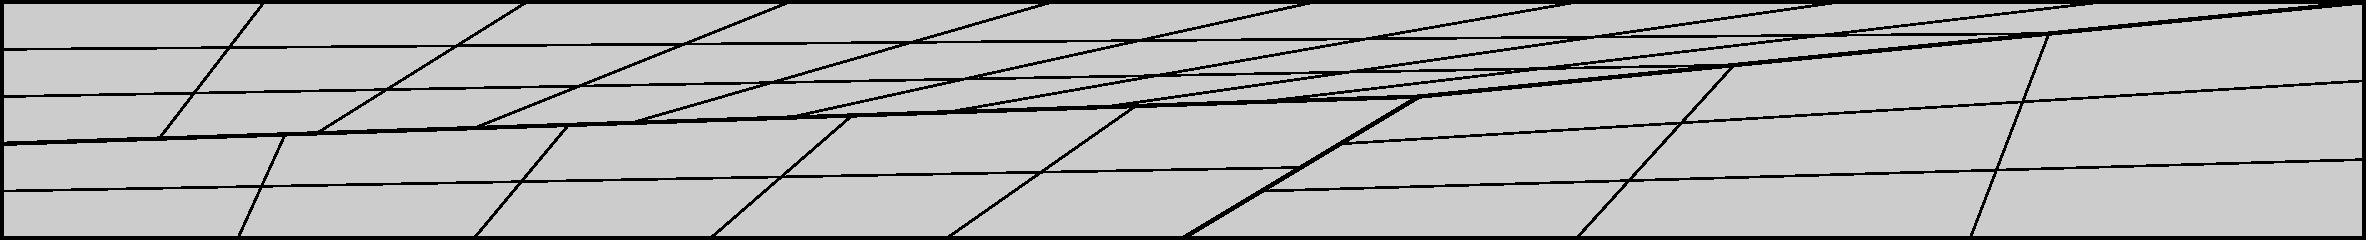
\includegraphics[width=\textwidth]{pure_shear_shell_mesh}
				\caption{}
				\label{fig:cantilever_mesh}
			\end{subfigure}
		\end{tabular}
		 &
		\begin{subfigure}[b]{0.48\columnwidth}
			\centering
			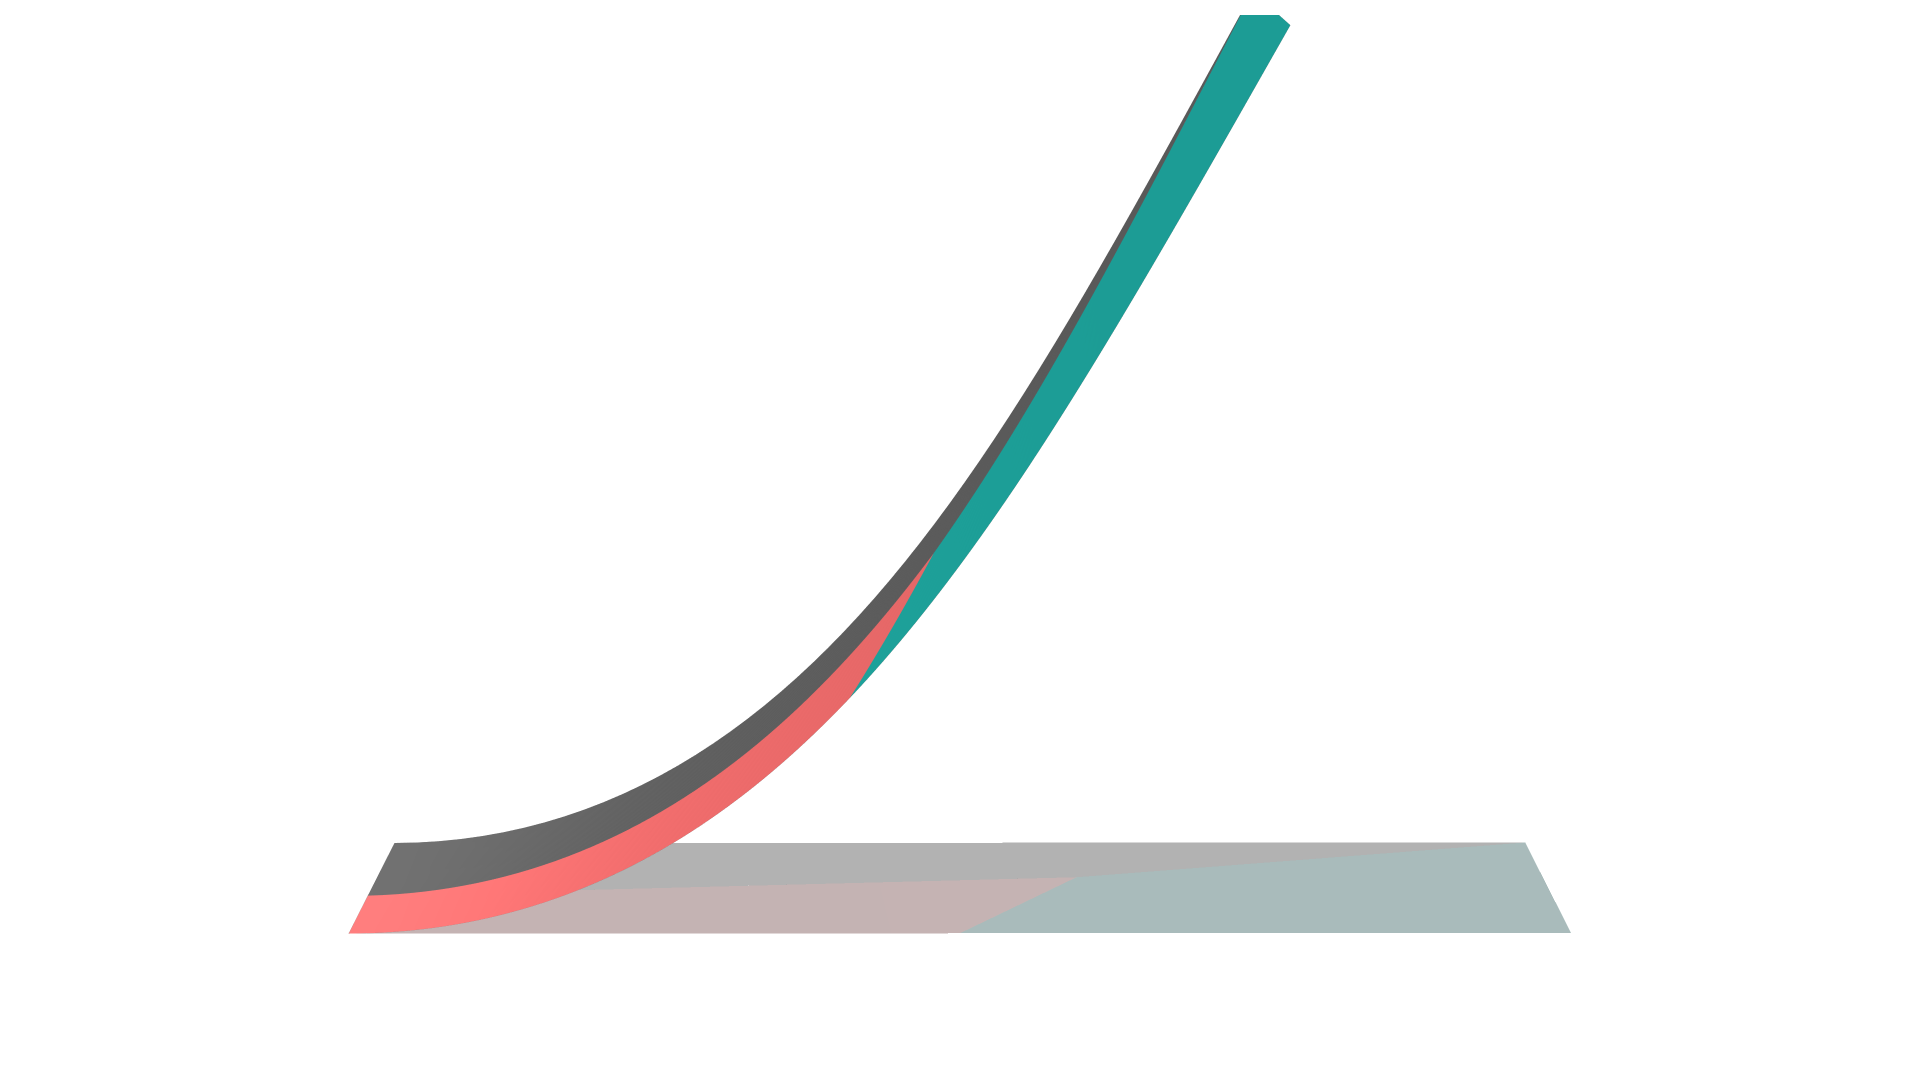
\includegraphics[width=\textwidth,scale=.26,trim={4cm 4cm 4cm 1cm},clip]{pure_shear_shell_deformed}
			\caption{}
			\label{fig:cantilever_deform}
		\end{subfigure}
	\end{tabular}
	% \label{fig:ABC}
	\caption{A cantilever subjected to an end shear force: (a) the problem description, (b) the three-patch non-matching discretization and (c) the initial and deformed configurations.}
\end{figure}

Figure~\ref{fig:cantilever_shear_result} shows the shear traction against the horizontal ($-u_x$) and vertical ($u_z$) displacements at the free end for both the non-conforming multi-patch configuration and the reference results reported by Sze et al.~\cite{sze2004popular}. Due to the heavy distortion of the mesh, the results are as expected poor for quadratic elements. However, the results for cubic splines agree with the reference result even for the coarse mesh. For all tested cases, the difference between the results obtained from the enriched \Bezier dual basis and the global dual basis are negligible.

\begin{figure}[h]
	\center
	\begin{subfigure}[b]{0.47\textwidth}
		\centering
		\includestandalone[scale=.8]{cantilever_shear_Q2_R0}
		\caption{}
	\end{subfigure}
	\begin{subfigure}[b]{0.47\textwidth}
		\centering
		\includestandalone[scale=.8]{cantilever_shear_Q2_R1}
		\caption{}
	\end{subfigure}
	\\
	\begin{subfigure}[b]{0.47\textwidth}
		\centering
		\includestandalone[scale=.8]{cantilever_shear_Q3_R0}
		\caption{}
	\end{subfigure}
	\begin{subfigure}[b]{0.47\textwidth}
		\centering
		\includestandalone[scale=.8]{cantilever_shear_Q3_R1}
		\caption{}
	\end{subfigure}
	\caption{Load-deflection curves for cantilever subjected to an end shear force. The horizontal ($-u_x$) and vertical ($u_z$) displacements at the free end for (a) a quadratic coarse mesh, (b) a quadratic fine mesh, (c) a cubic coarse mesh and (d) a cubic fine mesh are compared to the results provided in~\cite{sze2004popular}. }
	\label{fig:cantilever_shear_result}
\end{figure}
\FloatBarrier
\subsubsection{Slit annular plate subjected to a lifting line force}

In the second example, we study a slit annular plate subjected to a lifting line force. The problem setup is illustrated in Figure~\ref{fig:annular_shear_config}, where the inner radius, outer radius, thickness, maximum vertical traction load and load step are $R_0 = 6$, $R_1 = 10$, $t = 0.03$, $f = 0.8$ and $\Delta f = 0.04$, respectively. Young's modulus is $E = 21\times 10^6$ and Poisson's ratio is $0$. One end of the slit is fully clamped while the other end is lifted under the uniform traction load $f$. We benchmark the vertical displacements of points A and B. To test the performance of the proposed coupling formulation, we decompose the annular plate into three NURBS patches with $6\times 2$, $6\times 5$ and $6\times 3$ elements, respectively (see Figure~\ref{fig:annular_shear_mesh}). In this example, we also consider a fine mesh obtained by a uniform refinement of the mesh in Figure~\ref{fig:annular_shear_mesh}. The deformed annular plate is shown in Figure~\ref{fig:annular_shear_deform}.

% \begin{figure}[h]
% 	\center
% 	\begin{subfigure}[b]{.33\textwidth}
% 		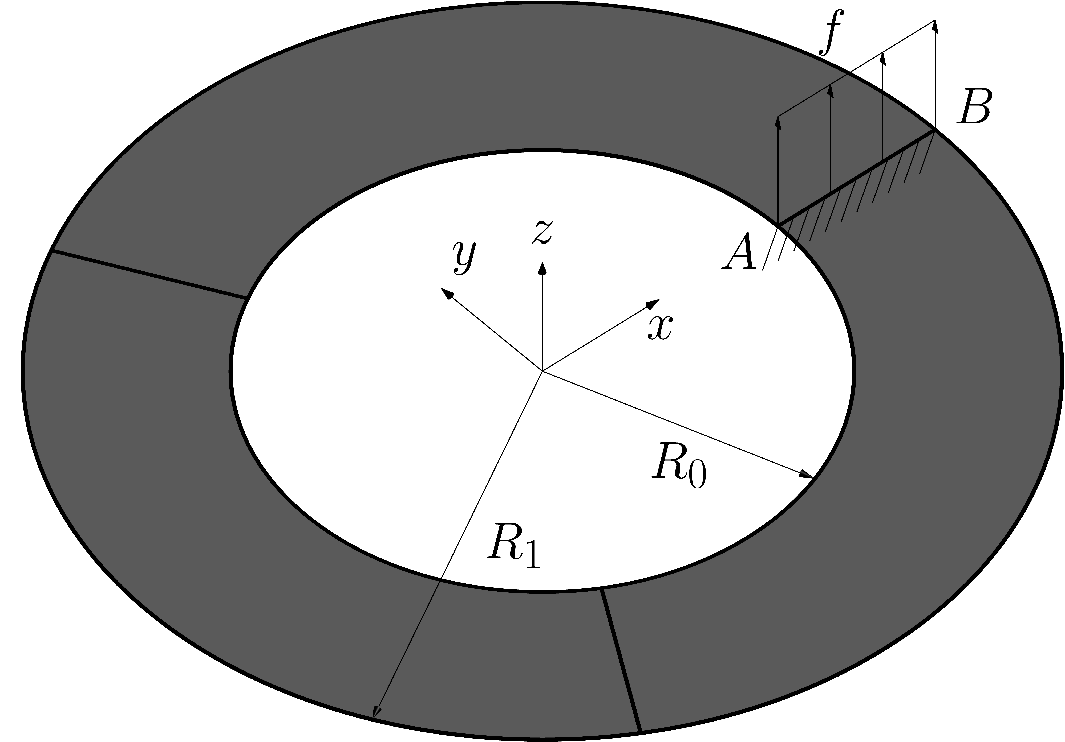
\includegraphics[scale=.35]{pure_shear_annular_config}
% 		\caption{}\label{fig:annular_shear_config}
% 	\end{subfigure}
% 	\begin{subfigure}[b]{.33\textwidth}
% 		\centering
% 		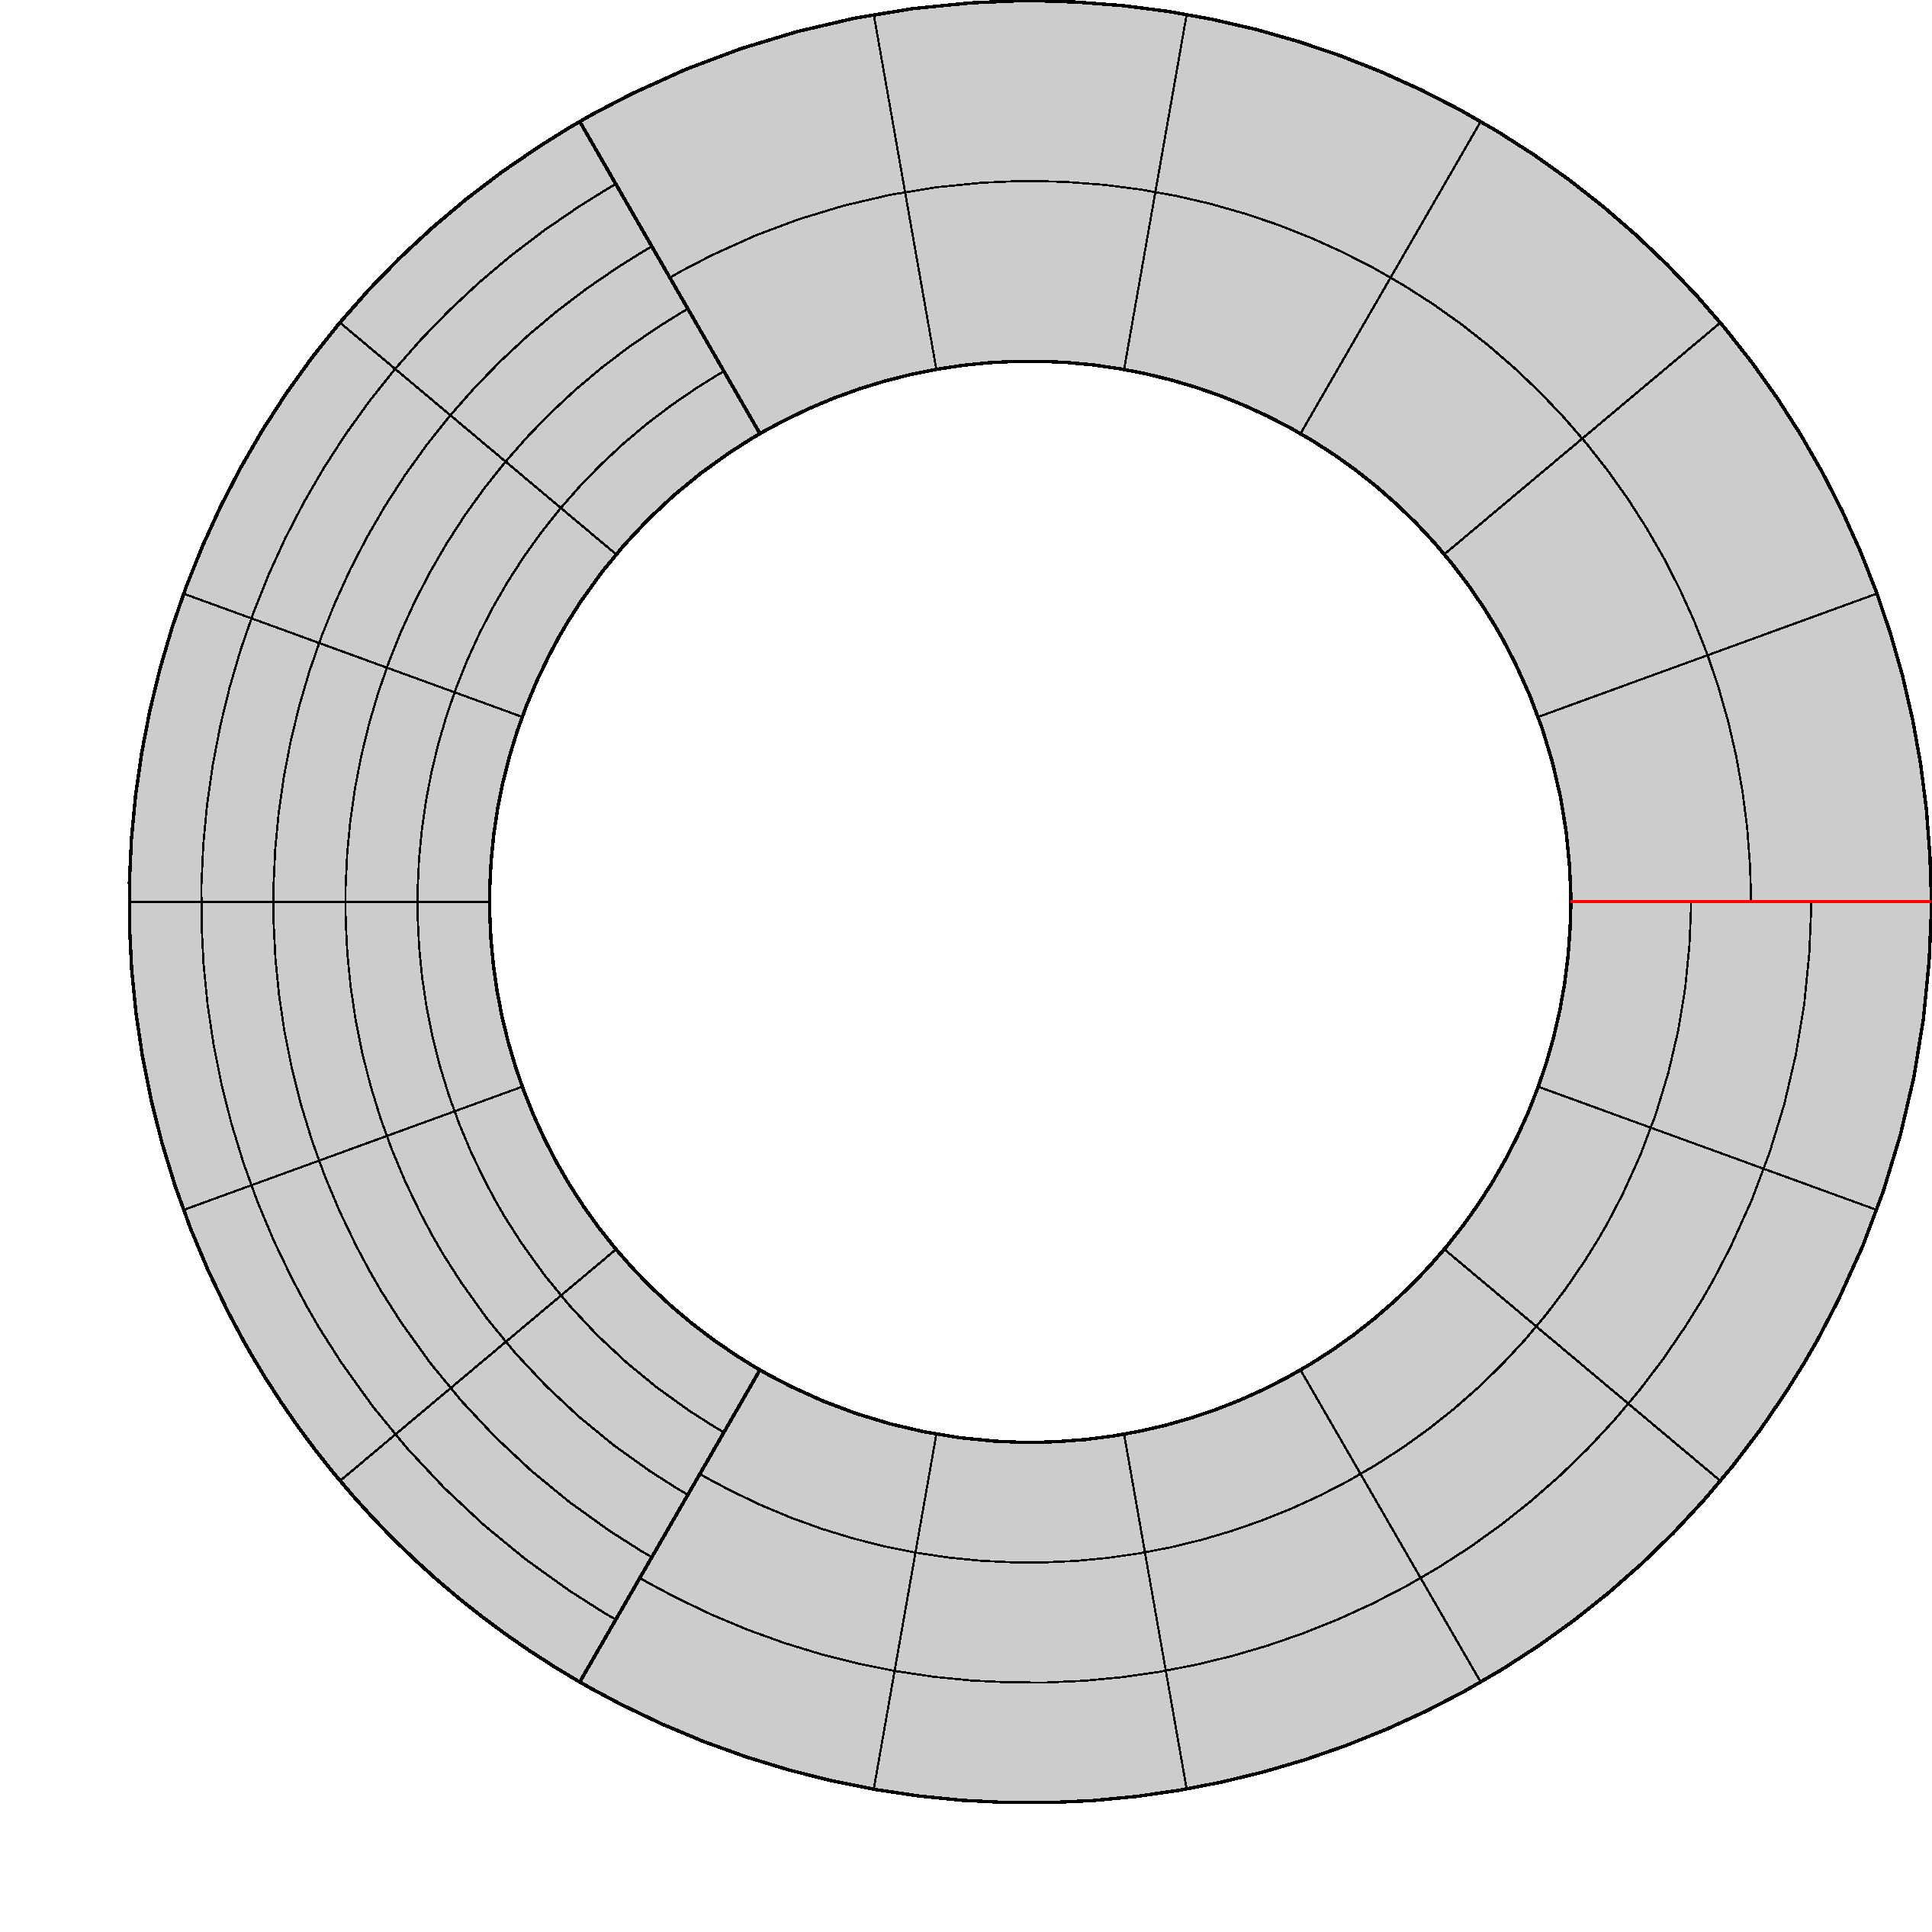
\includegraphics[scale=.13]{annular_mesh_2}
% 		\caption{}\label{fig:annular_shear_mesh}
% 	\end{subfigure}
% 	\begin{subfigure}[b]{.33\textwidth}
% 		\centering
% 		
\includegraphics[scale=.2,trim={16cm 4cm 16cm .5cm},clip]{annular_deformed}
% 		\caption{}\label{fig:annular_shear_deform}
% 	\end{subfigure}
% 	\caption{Slit annular plate subjected to a lifting line force: (a) the problem description, (b) the three-patch non-conforming discretization and (c) the initial and deformed configurations.}
% \end{figure}

\begin{figure}[h]
	\begin{tabular}[b]{cc}
		\begin{tabular}[b]{c}
			\begin{subfigure}[b]{0.4\columnwidth}
				\center
				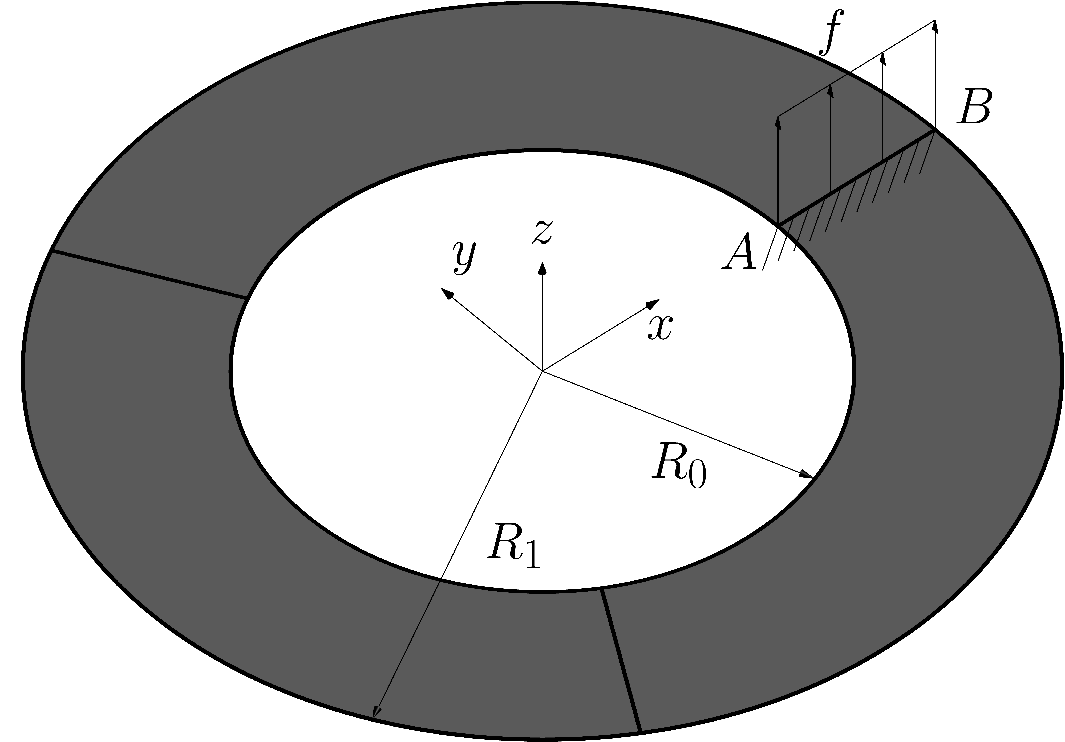
\includegraphics[width=.9\textwidth]{pure_shear_annular_config}
				\caption{}
				\label{fig:annular_shear_config}
			\end{subfigure} \\
			\begin{subfigure}[b]{0.4\columnwidth}
				\center
				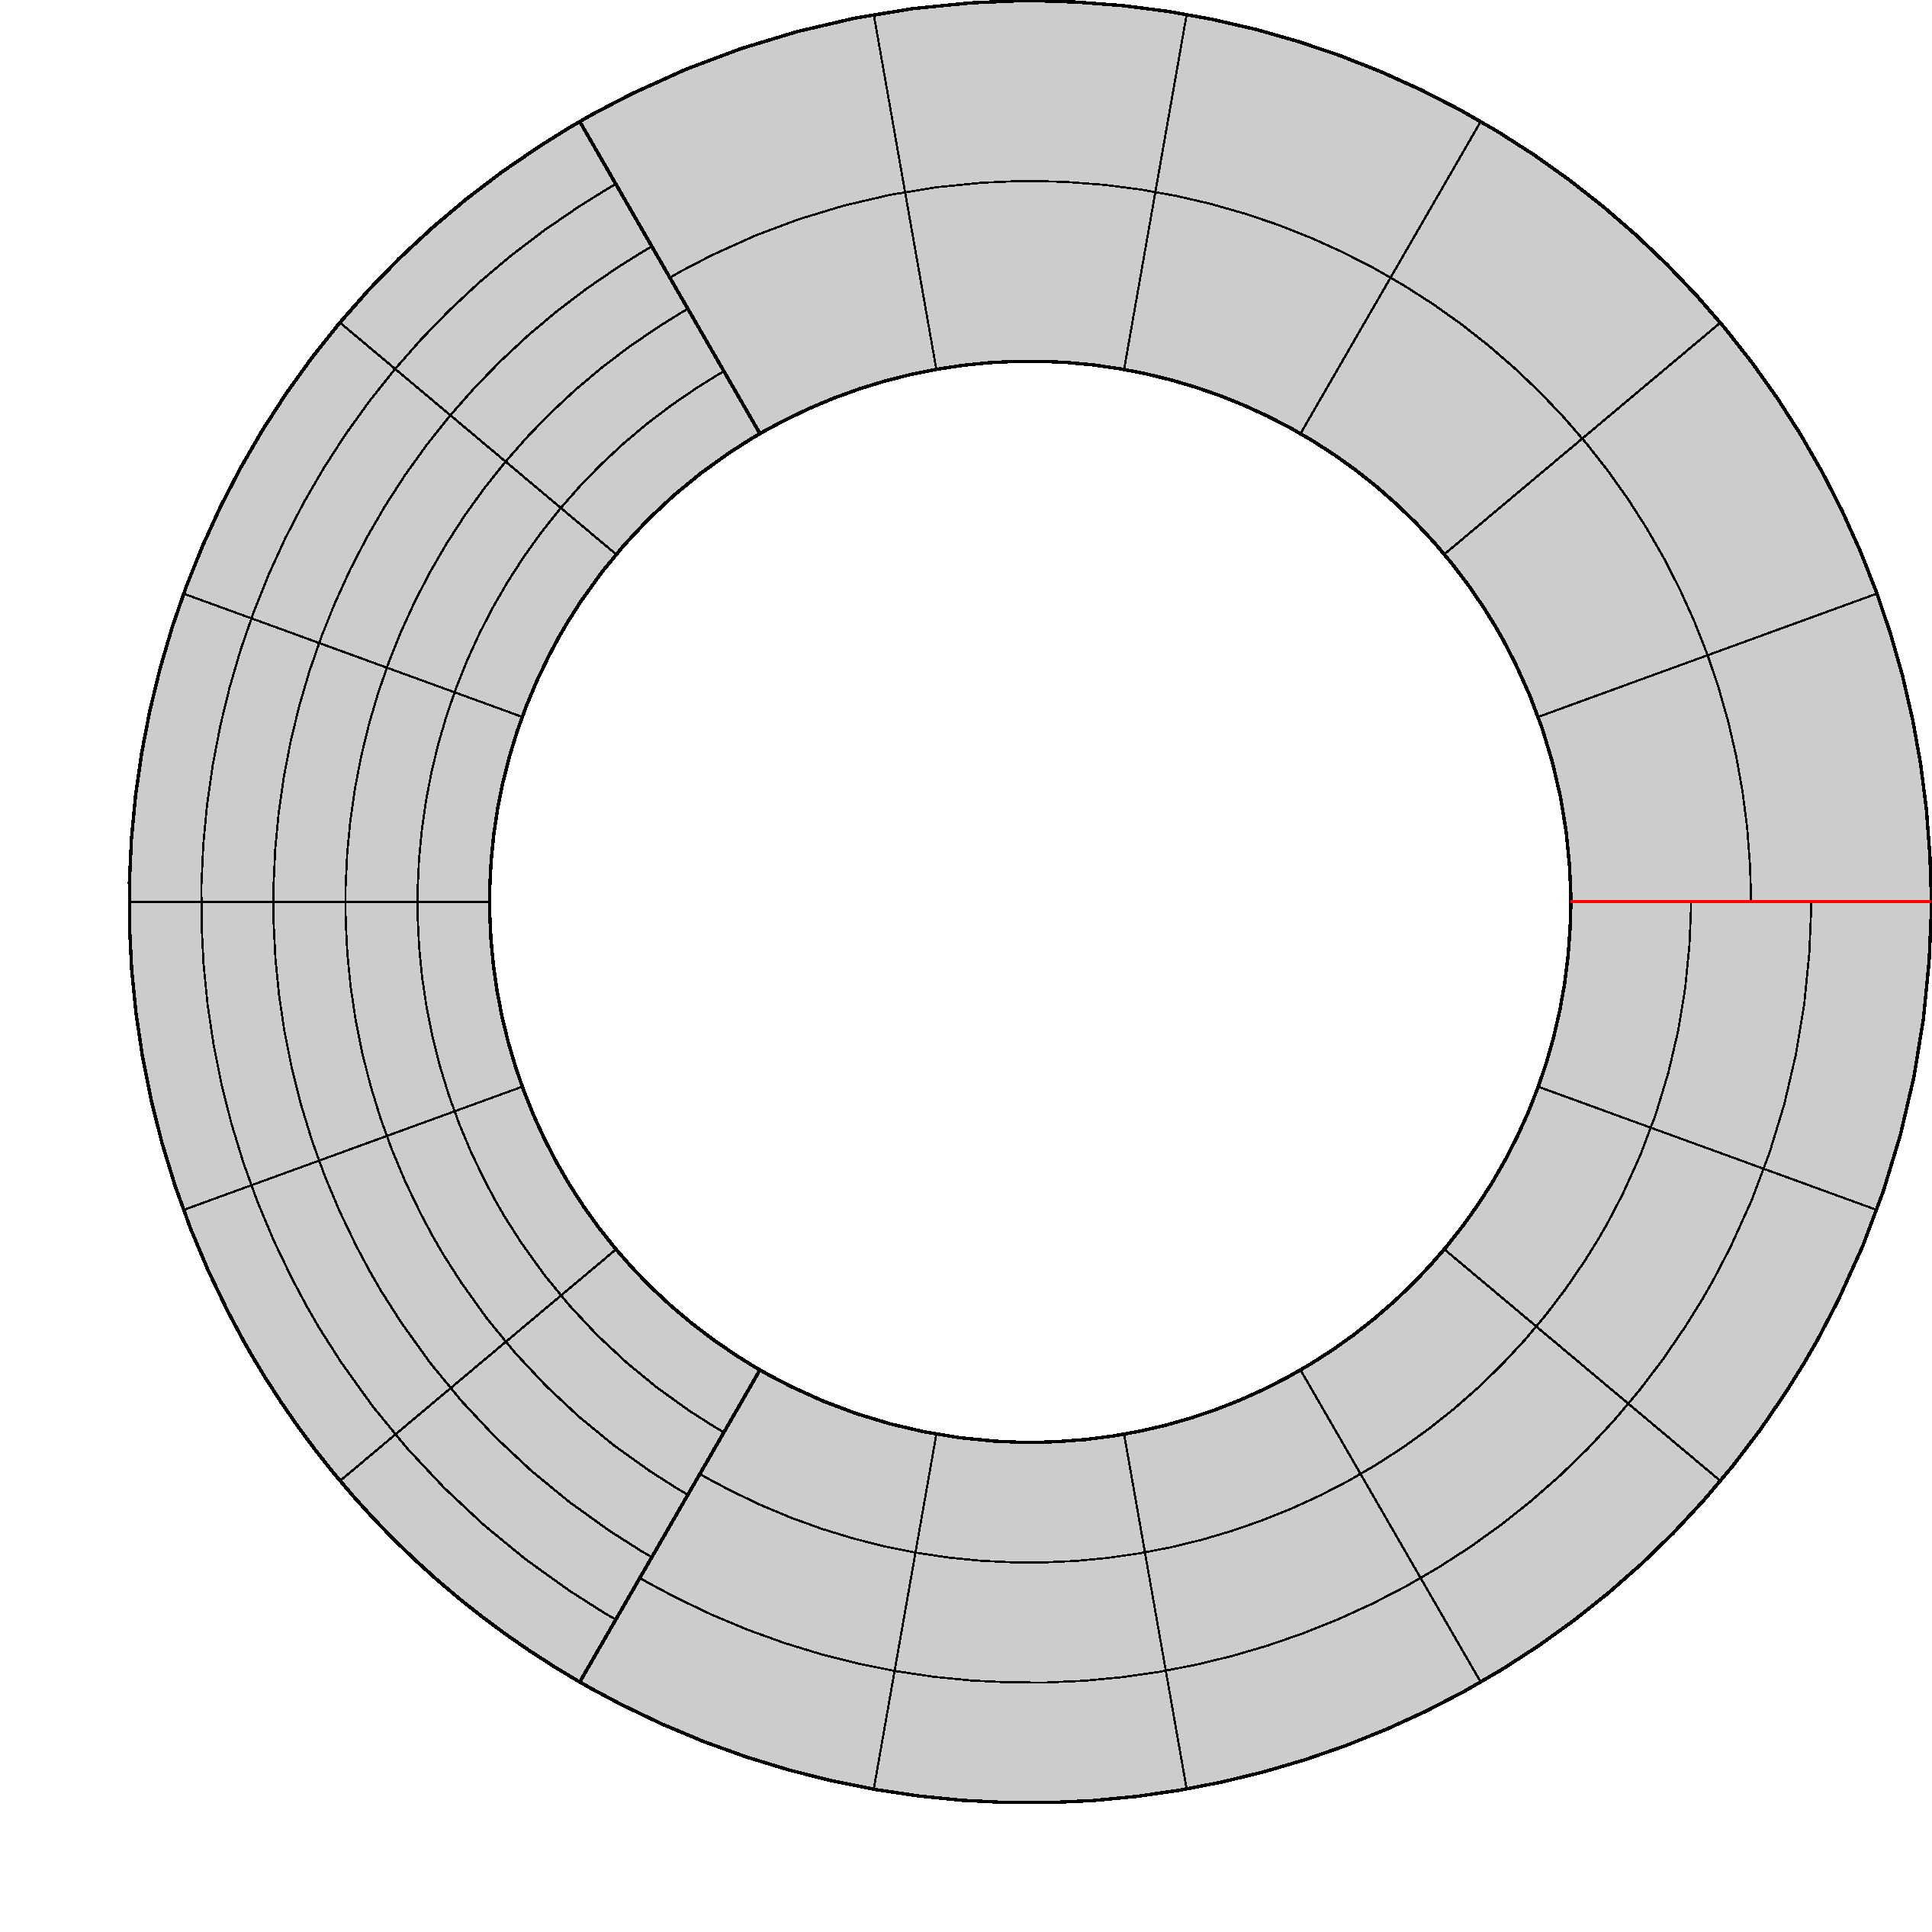
\includegraphics[width=.9\textwidth]{annular_mesh_2}
				\caption{}
				\label{fig:annular_shear_mesh}
			\end{subfigure}
		\end{tabular}
		 &
		\begin{subfigure}[b]{0.58\columnwidth}
			\center
			
\includegraphics[scale=.27,trim={17cm 4cm 17cm .5cm},clip]{annular_deformed}
			\caption{}
			\label{fig:annular_shear_deform}
		\end{subfigure}
	\end{tabular}
	% \label{fig:ABC}
	\caption{A cantilever subjected to an end shear force: (a) the problem description, (b) the three-patch non-matching discretization and (c) the initial and deformed configurations.}
\end{figure}

Figure~\ref{fig:annular_shear_result} shows the load against the vertical deflections of points A and B for both the non-conforming multi-patch configuration and the reference results provided in~\cite{sze2004popular}. Cubic elements are utilized in all tested cases. Whereas the multi-patch results obtained from the coarse mesh demonstrate slight discrepancy from the reference results, a good agreement with the reference results is observed for the fine mesh. Again, the difference between the results obtained from the enriched \Bezier dual basis and the global dual basis are negligible.

\begin{figure}[h]
	\center
	\begin{subfigure}[b]{.48\textwidth}
		\centering
		\includestandalone[scale=.8]{annular_shear_Q3_R0}
		\caption{}
	\end{subfigure}
	\begin{subfigure}[b]{.48\textwidth}
		\centering
		\includestandalone[scale=.8]{annular_shear_Q3_R1}
		\caption{}
	\end{subfigure}
	\caption{Load-deflection curves for the slit annular plate lifted by a lifting line force. The vertical displacements at tip A and B for (a) a cubic coarse mesh and (b) a cubic fine mesh are compared to the results provided in~\cite{sze2004popular}. }
	\label{fig:annular_shear_result}
\end{figure}
\FloatBarrier
\subsubsection{Pullout of an open-ended cylindrical shell}

In this test, an open-ended cylinder is pulled by a pair of radial forces. The problem setup is illustrated in Figure~\ref{fig:cylindrical_pull_config}, where the radius, length, thickness of the cylinder, radial force and load step are $R = 4.953$, $L = 10.35$, $t = 0.094$, $P = 40,000$ and $\Delta P = 1,000$, respectively. The material properties are: Young's modulus $E = 10.5\times 10^6$ and Poisson's ratio $\nu = 0.3125$. We benchmark $u_z$ at point A, $u_x$ and points B and C, correspondingly. The cylindrical shell is modeled by four NURBS patches, discretized by $32\times 16$, $28\times 14$, $28\times 14$ and $32\times 16$, respectively (see Figure~\ref{fig:cylindrical_pull_config}). The results of Sze et al.~\cite{sze2004popular} are used as the reference. A good agreement with the reference results is observed in Figure~\ref{fig:cylindrical_pull_result} indicating the accuracy and robustness of our formulation.

\begin{figure}[h]
	\center
	\begin{subfigure}[b]{\textwidth}
		\centering
		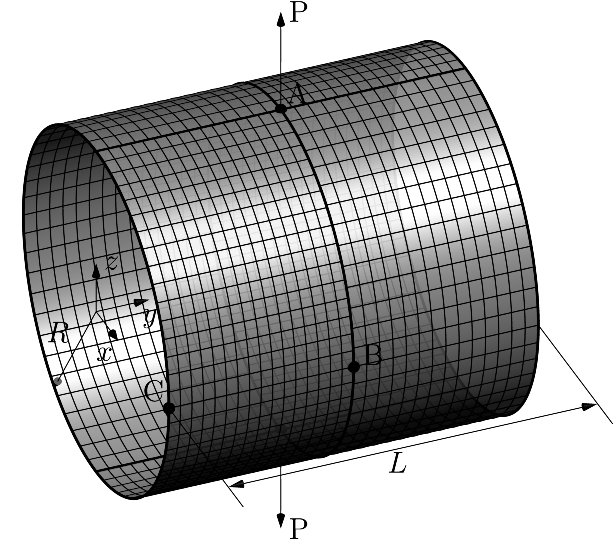
\includegraphics[width=.6\textwidth]{cylindrical_configuration}
		% \begin{tikzpicture}
		% 	% \node[inner sep=0pt] at (0,0)
		% 	{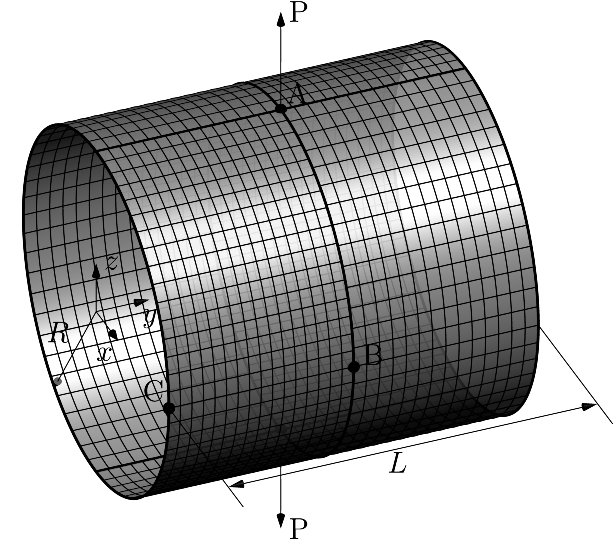
\includegraphics[width=.6\textwidth]{cylindrical_configuration}};
		% 	% \node[draw,align=left] at (7.2,0) {$E=10.5\times 10^6$\\$R=4.953$\\$\nu=0.3125$\\$L=10.35$\\$h=0.094$\\$P=40000$};
		% \end{tikzpicture}
		\caption{}\label{fig:cylindrical_pull_config}
	\end{subfigure}
	\\\hspace{1em}
	\begin{subfigure}[b]{.47\textwidth}
		\centering
		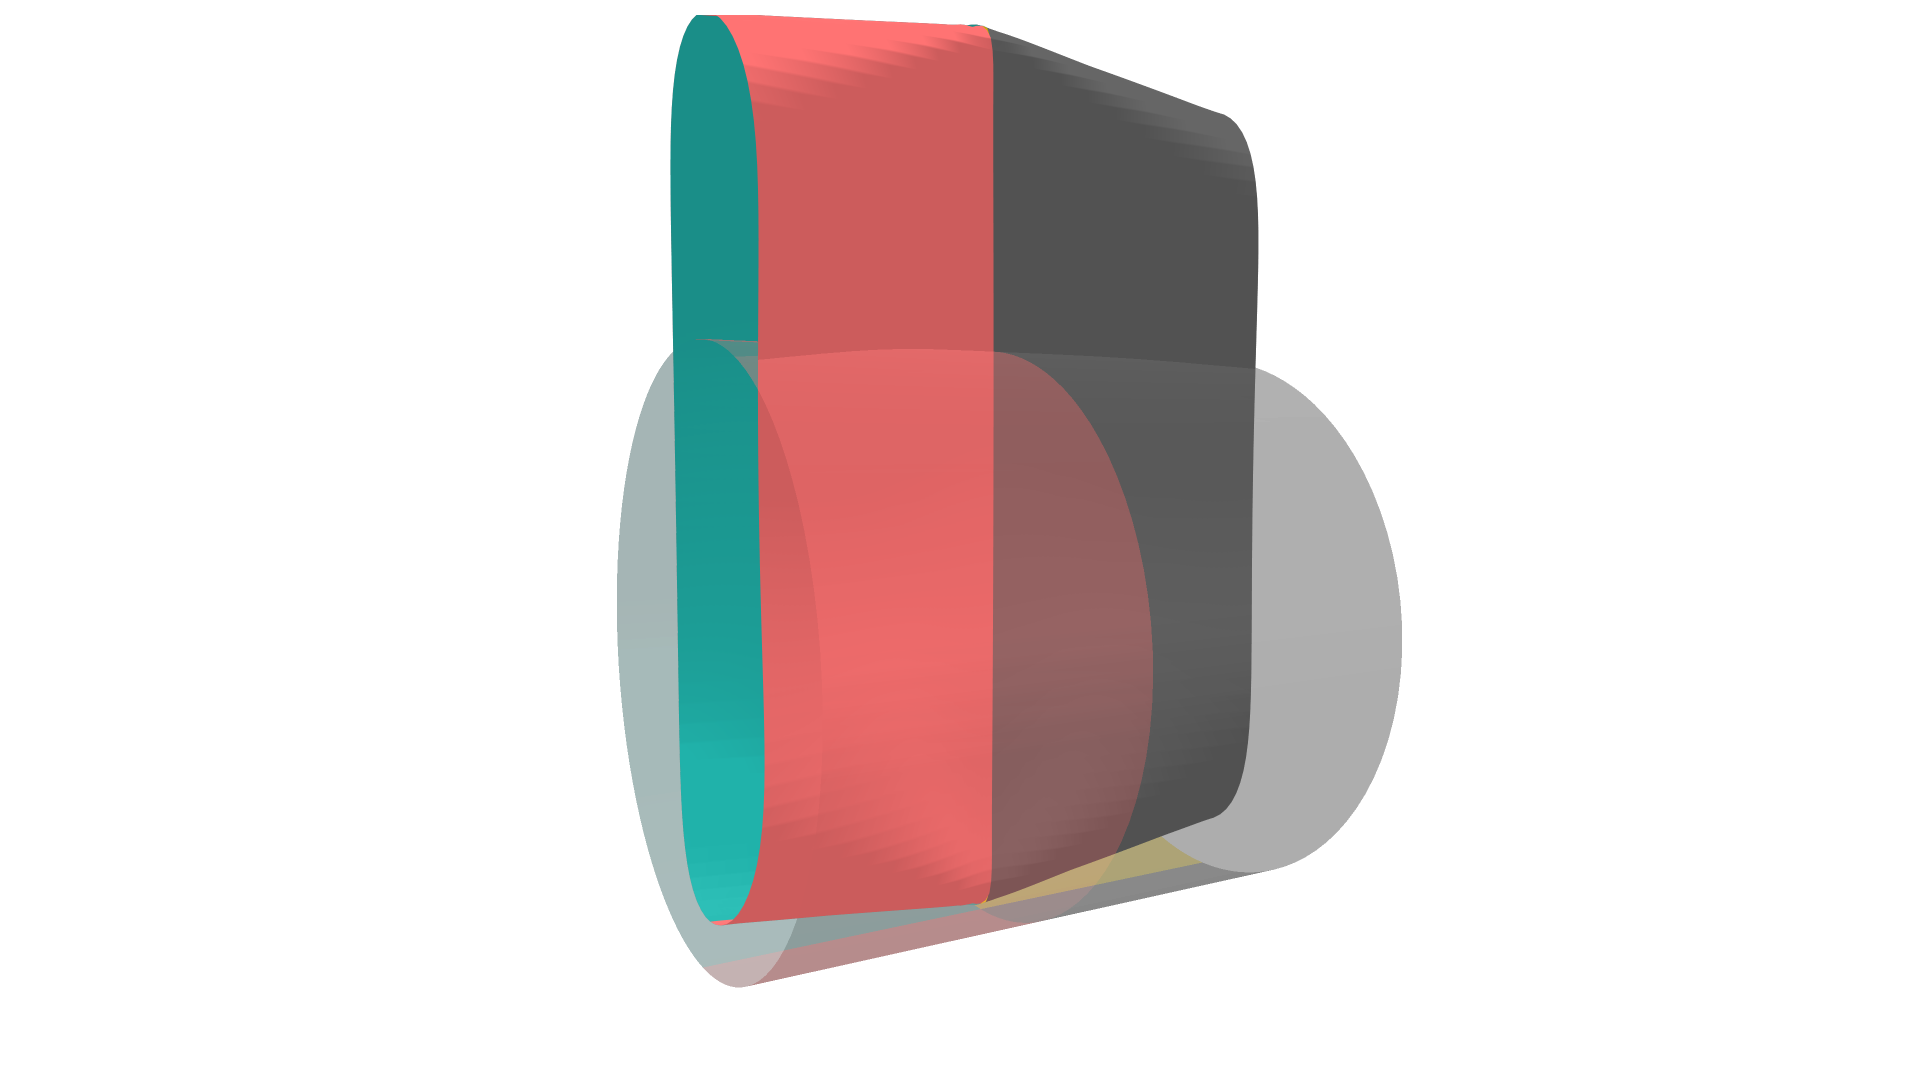
\includegraphics[scale=.2,trim={18cm 3cm 18cm 0cm},clip]{cylindrical_deformed}
		\caption{}
	\end{subfigure}
	\begin{subfigure}[b]{.47\textwidth}
		\centering
		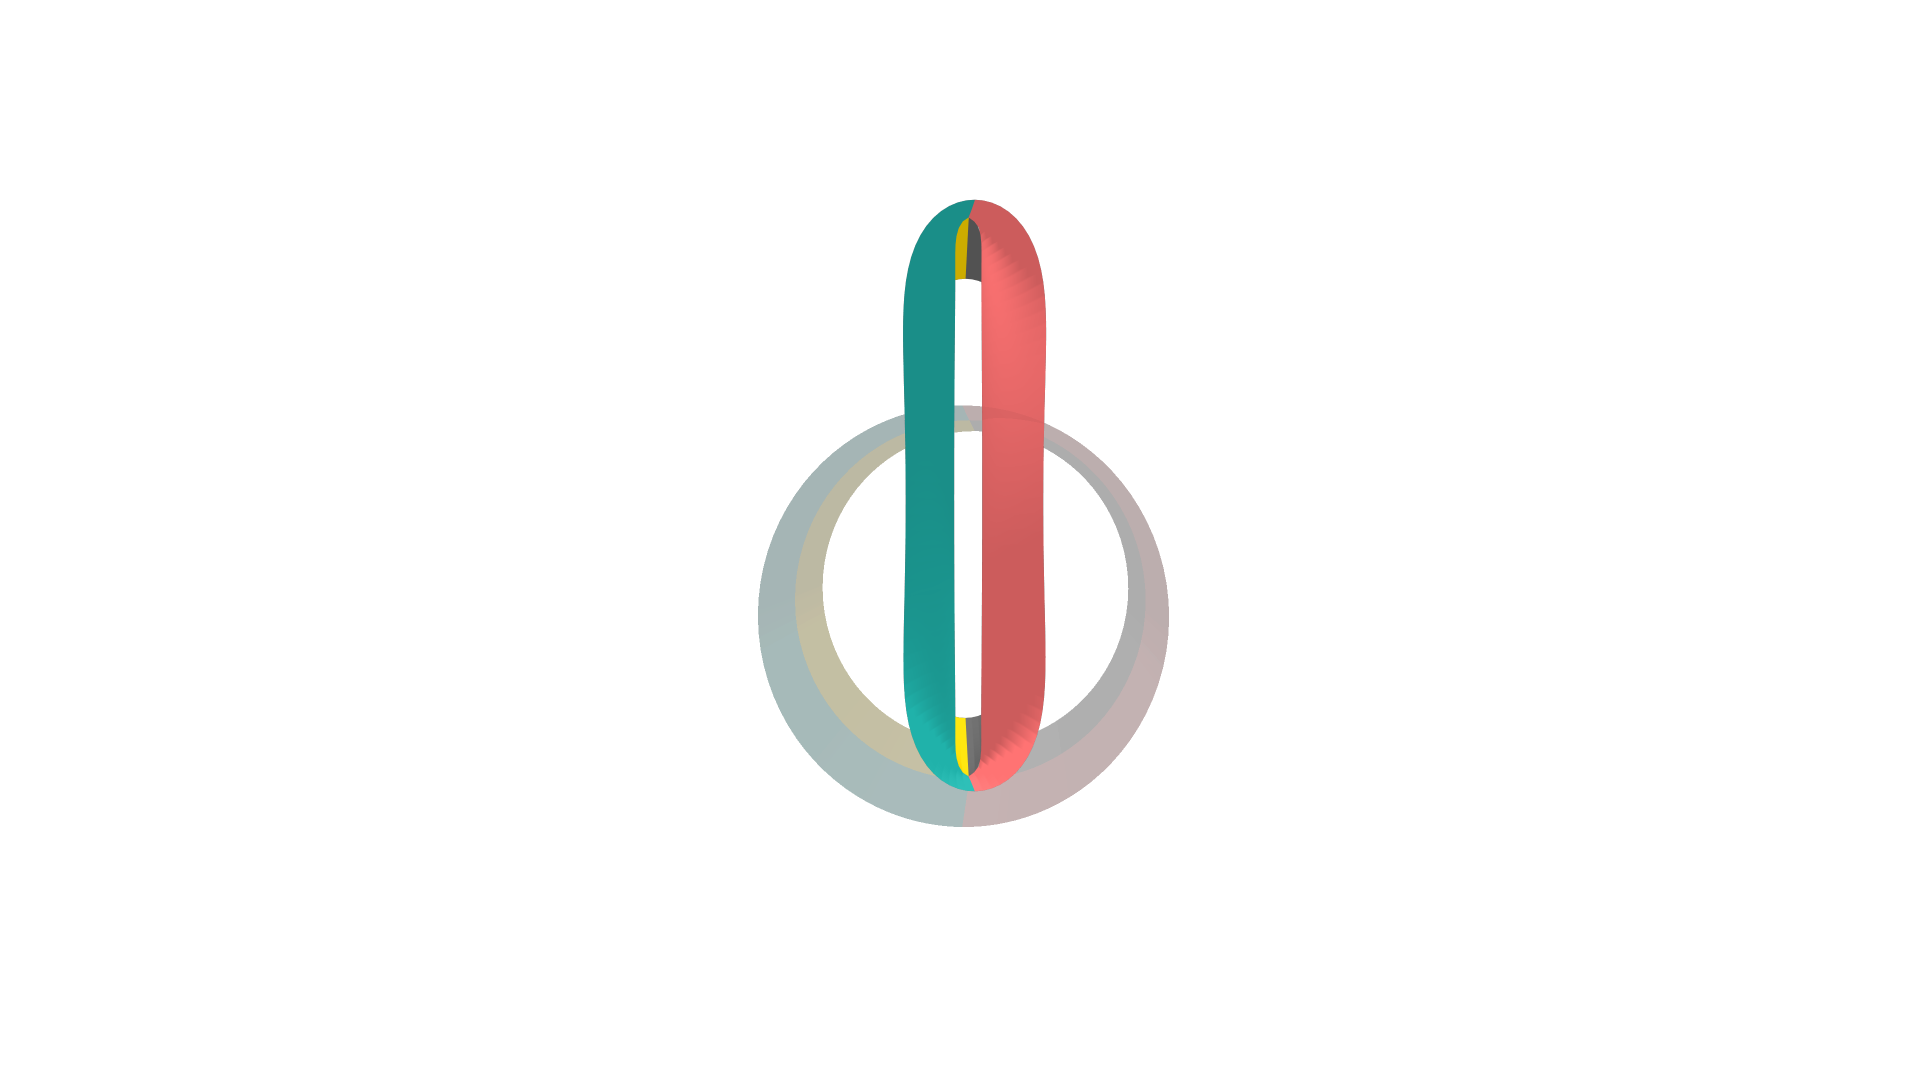
\includegraphics[scale=.3,trim={22cm 8cm 22cm 3cm},clip]{cylindrical_deformed_2}
		\caption{}
	\end{subfigure}
	\caption{The open-end cylindrical shell subjected to radial pulling forces: (a) the problem description and four-patch non-matching discretization, (b) the initial and deformed configurations in 3D view, and (c) the initial and deformed configurations in $y$-axis view.}

\end{figure}

\begin{figure}[ht]
	\center
	\centering
	\includestandalone[scale=.8]{cylindrical_shell_pull_Q3}
	\caption{Load-deflection curves of the open-end cylinder subjected to a point pulling load. The results are measured at points A, B and C.}
	\label{fig:cylindrical_pull_result}
\end{figure}

\FloatBarrier

\section{Conclusion}\label{sec:conlusion}
In this chapter, we present a dual mortar formulation for the Kirchhoff-Love shell problem. The proposed formulation is based on the enriched \Bezier dual basis and generic dual-compatible constraints. The enriched \Bezier dual basis reproduces polynomial up to a given order without losing its locality. Thanks to the dual-compatible constraint, the biorthogonality between the dual basis functions and the corresponding primal spline basis functions can be extended to the discretized constraint matrix. Hence, the static condensation can be achieved without extra computational effort. With the help of the enriched \Bezier dual basis, the condensed linear system remains sparse. Moreover, the constraint utilized in our formulation is generic in the sense that it handles $C^1$ continuity for smooth shell coupling as well as angle preservation for patches joined at a kink. When kinks present, the constraint is no longer linear. Thus, Newton-Raphson iteration is needed in order to apply the constraint. Due to the presence of the residual of the constraint, the linearized constraint is non-homogeneous. Thanks to the unique constraint matrix structure, a particular solution that satisfies the non-homogeneous constraints can be constructed without the need to solve any linear systems. \par

The accuracy and robustness of the proposed formulation are verified by several linear and nonlinear benchmark problems. The Kirchhoff plate and Scordelis-Lo roof problems indicate the optimality of the proposed formulation. The T-beam and L-beam problems demonstrate the ability of the proposed formulation in preserving coupling anlge. From the benchmark results, we believe the proposed patch coupling formulation has great potential in addressing real world complex shell problems.